%Lovingly retyped by Akram S. Sadek, a.sadek@physics.org, 22 March 2005

\documentclass[twocolumn,preprintnumbers,amsmath,amssymb,floatfix]{revtex4}
\usepackage{graphicx}	% Include figure files
\usepackage{dcolumn}	% Align table columns on decimal point
\usepackage{bm}		% bold math
\usepackage{amsmath}

\graphicspath{{figures/}}	% Setting the graphicspath

\begin{document}

\bibliographystyle{unsrt}

\title{Probabilistic logics and the synthesis
of reliable\\ organisms from unreliable components}

\author{J. von Neumann}

\date{1956, Lectures delivered at the California Institute of Technology, January 1952}

\begin{abstract}
\noindent In C. E. Shannon and J. McCarthy, editors,
\emph{Automata Studies}, pp. 329-378. Princeton University Press,
Princeton, NJ, 1956.
\end{abstract}

\maketitle

\section{\label{sec:one}Introduction}

The paper that follows is based on notes taken by Dr. R. S. Pierce
on five lectures given by the author at the California Institute
of Technology in January 1952. They have been revised by the
author but they reflect, apart from minor changes, the lectures as
they were delivered.

The subject-matter, as the title suggests, is the role of error in
logics, or in the physics implementation of logics - in
automata-synthesis. Error is viewed, therefore, not as an
extraneous and misdirected or misdirecting accident, but as an
essential part of the process under consideration - its importance
in the synthesis of automata being fully comparable to that of the
factor which is normally considered, the intended and correct
logical structure.

Our present treatment of error is unsatisfactory and ad hoc. It is
the author's conviction, voiced over many years, that error should
be treated by thermodynamical methods, and be the subject of a
thermodynamical theory, as information has been, by the work of L.
Szilard and C. E. Shannon [Cf. \ref{sec:five2}]. The present
treatment falls far short of achieving this, but it assembles, it
is hoped, some of the building materials, which will have to enter
into the final structure.

The author wants to express his thanks to K. A. Brueckner and M.
Gell-Mann, then at the University of Illinois, to whose
discussions in 1951 he owes some important stimuli on this
subject; to Dr. R. S. Pierce at the California Institute of
Technology, on whose excellent notes this exposition is based; and
to the California Institute of Technology, whose invitation to
deliver these lectures combined with the very warm reception by
the audience, caused him to write this paper in its present form,
and whose cooperation in connection with the present publication
is much appreciated.

\section{\label{sec:two}A Schematic View of Automata}

\subsection{\label{sec:two1}Logics and Automata}

It has been pointed out by A. M. Turing \cite{Turing36} in 1937
and by W. S. McCulloch and W. Pitts \cite{McCulloch43} in 1943
that effectively constructive logics, that is, intuitionistic
logics, can be best studied in terms of automata. Thus logical
propositions can be represented as electrical networks or
(idealized) nervous systems. Whereas logical propositions are
built up by combining certain primitive symbols, networks are
formed by connecting basic components, such as relays in
electrical circuits and neurons in the nervous system. A logical
proposition is then represented as a ``black box" which has a
finite number of inputs (wires or nerve bundles) and a finite
number of outputs. The operation performed by the box is
determined by the rules defining which inputs, when stimulated,
cause responses in which outputs, just as a propositional function
is determined by its values for all possible assignments of values
to its variables.

There is one important difference between ordinary logic and the
automata which represent it. Time never occurs in logic, but every
network or nervous system has a definite time lag between the
input signal and the output response. A definite temporal sequence
is always inherent in the operation of such a real system. This is
not entirely a disadvantage. For example, it prevents the
occurrence of various kinds of more or less overt vicious circles
(related to ``non-constructivity", ``impredicativity", and the
like) which represent a major class of dangers in modern logical
systems. It should be emphasized again, however, that the
representative automaton contains more than the content of the
logical proposition which it symbolizes - to be precise, it
embodies a definite time lag.

Before proceeding to a detailed study of a specific model of
logic, it is necessary to add a word about notation. The
terminology used in the following is taken from several fields of
science; neurology, electrical engineering, and mathematics
furnish most of the words. No attempt is made to be systematic in
the application of terms, but it is hoped that the meaning will be
clear in every case. It must be kept in mind that few of the terms
are being used in the technical sense which is given to them in
their own scientific field. Thus, in speaking of a neuron, we
don't mean the animal organ, but rather one of the basic
components of our network which resembles an animal neuron only
superficially, and which might equally well have been called an
electrical relay.

\subsection{\label{sec:two2}Definitions of the Fundamental Concepts}

Externally an automaton is a ``black box" with a finite number of
inputs and a finite number of outputs. Each input and each output
is capable of exactly two states, to be designated as the
``stimulated" state and the ``unstimulated" state, respectively.
The internal functioning of such a ``black box" is equivalent to a
prescription that specifies which outputs will be stimulated in
response to the stimulation of any given combination of the
inputs, and also the time of stimulation of these outputs. As
stated above, it is definitely assumed that the response occurs
only after a time lag, but in the general case the complete
response may consist of a succession of responses occurring at
different times. This description is somewhat vague. To make it
more precise it will be convenient to consider first automata of a
somewhat restricted type and to discuss the synthesis of the
general automaton later.\\

\noindent \textsc{Definition 1:} A single output automaton with
time delay $\delta$ ($\delta$ is positive) is a finite set of
inputs, exactly one output, and an enumeration of certain
``preferred" subunits of the set of all inputs. The automaton
stimulates its output at time $t+\delta$ if and only if at time
$t$ the stimulated inputs constitute a subset which appears in the
list of ``preferred" subsets, describing the automaton.\\

In the above definition the expression ``enumeration of certain
subsets" is taken in its widest sense and does not exclude the
extreme cases ``all" and ``none". If $n$ is the number of inputs,
then there exist $2^{(2^n)}$ such automata for any given $\delta$.

Frequently several automata of thus type will have to be
considered simultaneously. They need not all have the same time
delay, but it will be assumed that all their time lags are
integral multiples of a common value $\delta_0$. This assumption
may not be correct for an actual nervous system; the model
considered may apply only to an idealized nervous system. In
partial justification, it can be remarked that as long as only a
finite number of automata are considered, the assumption of a
common value $\delta_0$ can be realized within any degree of
approximation. Whatever its justification and whatever its meaning
in relation to actual machines or nervous systems, this assumption
will be made in our present discussions. The common value
$\delta_0$ is chosen for convenience as the time unit. The time
variable can now be made discrete, i.e., it need assume only
integral numbers as values, and correspondingly the time delays of
the automata considered are positive integers.

Single output automata with given time delays can be combined into
a new automaton. The outputs of certain automata are connected by
lines or wires or nerve fibres to some of the inputs of the same
or other automata. The connecting lines are used only to indicate
the desired connections; their function is to transmit the
stimulation of an output instantaneously to all the inputs
connected with that output. The network is subjected to one
condition, however. Although the same output may be connected to
several inputs, any one input is assumed to be connected to at
most one output. It may be clearer to impose this restriction on
the connecting lines, by requiring that each input and each output
be attached to exactly one line, to allow lines to be split into
several lines, but prohibit the merging of two or more lines. This
convention makes it advisable to mention again that the activity
of an output or an input, and hence of a line, is an all or
nothing process. If a line is split, the stimulation is carried to
all the branches in full. No energy conservation laws enter into
the problem. In actual machines or neurons, the energy is supplied
by the neurons themselves from some external source of energy. The
stimulation acts only as a trigger device.

The most general automaton is defined to be any such network. In
general it will have several inputs and several outputs and its
response activity will be much more complex than that of a single
output automaton with a given time delay. An intrinsic definition
of the general automaton, independent of its construction as a
network, can be supplied. It will not be discussed here, however.

Of equal importance to the problem of combining automata into new
ones is the converse problem of representing a given automaton by
a network of simpler automata, and of determining eventually a
minimum number of basic types for these simpler automata. As will
be shown, very few types are necessary.

\subsection{\label{sec:two3}Some Basic Organs}

The automata to be selected as a basis for the synthesis of all
automata will be called basic organs. Throughout what follows,
these will be single output automata.

\begin{figure}

\includegraphics[width=2.4in]{fig_1}
\caption{\label{fig:1}}
\end{figure}

One type of basic organ is described by Figure~\ref{fig:1}. It has
one output, and may have any finite number of inputs. These are
grouped into two types: Excitatory and inhibitory inputs. The
excitatory inputs are distinguished from the inhibitory inputs by
the addition of an arrowhead to the former and of a small circle
to the latter. This distinction of inputs into two types does
actually not relate to the concept of inputs, it is introduced as
a means to describe the internal mechanism of the neuron. This
mechanism is fully described by the so-called threshold function
$\phi(x)$ written inside the large circle symbolizing the neuron
in Figure~\ref{fig:1}, according to the following convention: The
output of the neuron is excited at time $t+1$ if and only if at
time $t$ the number of stimulated excitatory inputs $k$ and the
number of stimulated inhibitory inputs $\ell$ satisfy the relation
$k\geq \phi(\ell)$. (It is reasonable to require that the function
$\phi(x)$ be monotone non-decreasing.) For the purposes of our
discussion of this subject it suffices to use only certain special
classes of threshold functions $\phi(x)$. E.g.

\begin{eqnarray}
\phi(x) = \psi_{h}(x) \left\{
\begin{array}{l}
=0\\
=\infty
\end{array}
\mathrm{~for~}
\begin{array}{r}
x < h\\
x \geq h
\end{array}\right\}
\label{eq:1}
\end{eqnarray}

\noindent (i.e., $<h$ inhibitions are absolutely ineffective,
$\geq h$ inhibitions are absolutely effective), or

\begin{equation}
\phi(x)=x_{h}(x)=x+h \label{eq:2}
\end{equation}

\noindent (i.e., the excess of stimulations over inhibitions must
be $\geq h$). We will use $x_{h}$, and write the inhibition number
$h$ (instead of $x_h$) inside the large circle symbolizing the
neuron. Special cases of this type are the three basic organs
shown in Figure~\ref{fig:2}. These are, respectively, a threshold
two neuron with two excitatory inputs, a threshold one neuron with
one excitatory input and one inhibitory input.

\begin{figure}
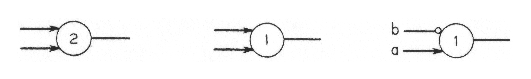
\includegraphics[width=3.4in]{fig_2}
\caption{\label{fig:2}}
\end{figure}

The automata with one output and one input described by the
networks shown in Figure~\ref{fig:3} have simple properties: The
first one's output is never stimulated, the second one's output is
stimulated at all times if its input has been ever (previously)
stimulated. Rather than add these automata to a network, we shall
permit lines leading to an input to be either always
non-stimulated, or always stimulated. We call the former
``grounded" and designate it by the symbol $~|~|~_\vdash~$ and we
call the latter ``live" and designate it by the symbol
$~|\shortmid|~_\vdash$~.

\begin{figure}[b]

\includegraphics[width=3.4in]{fig_3}
\caption{\label{fig:3}}
\end{figure}

\section{\label{sec:three}Automata and the Propositional Calculus}

\subsection{\label{sec:three1}The Propositional Calculus}

The propositional calculus deals with propositions irrespective of
their truth. The set of propositions is closed under the
operations of negation, conjunction and disjunction. If $a$ is a
proposition, then ``not a", denoted by $a^{-1}$ (we prefer this
designation to the more conventional ones $-a$ and $\sim{a}$), is
also a proposition. If $a$, $b$ are two propositions, then ``a and
b", ``a or b", denoted respectively by $ab$, $a+b$, are also
propositions. Propositions fall into two sets, T and F, depending
whether they are true or false. The proposition $a^{-1}$ is in T
if and only if $a$ is in F. The proposition $ab$ is in T if an
only if $a$ and $b$ is in T. Mathematically speaking the set of
propositions, closed under the three fundamental operations, is
mapped by a homomorphism onto the Boolean algebra of the two
elements $\underline{1}$ and $\underline{0}$. A proposition is
true if and only if it is mapped onto the element $\underline{1}$.
For convenience, denote by $\underline{1}$ the proposition
$\bar{a}+\bar{a}^{-1}$, by $\underline{0}$ the proposition
$\bar{a}\bar{a}^{-1}$, where $\bar{a}$ is a fixed but otherwise
arbitrary proposition. Of course, $\underline{0}$ is false and
$\underline{1}$ is true.

A polynomial $P$ in $n$ variables, $n \geq 1$, is any formal
expression obtained from $x_1, \ldots, x_n$ by applying the
fundamental operations to them a finite number of times, for
example $[(x_1 + x_2^{-1})x_3]^{-1}$ is a polynomial. In the
propositional calculus two polynomials in the same variables are
considered equal if and only if for any choice of the propositions
$x_1, \ldots, x_n$ the resulting two propositions are always
either both true or both false. A fundamental theorem of the
propositional calculus states that every polynomial $P$ is equal
to

\begin{equation*}
\sum_{i_1=\pm1} \ldots \sum_{i_n=\pm 1}f_{i_1 \ldots i_n}x_1^{i_1}
\cdots x_n^{i_n},
\end{equation*}

\noindent where each of the $f_{i_1 \ldots i_n}$ is equal to
$\underline{0}$ or $\underline{1}$. Two polynomials are equal if
and only if their $f$'s are equal. In particular, for each $n$,
there exist exactly $2^{(2^n)}$ polynomials.

\subsection{\label{sec:three2}Propositions, Automata and Delays}

These remarks enable us to describe the relationship between
automata and the propositional calculus. Given a time delay $s$,
there exists a one-to-one correspondence between single output
automata with time delay $s$ and the polynomials of the
propositional calculus. The number $n$ of inputs (to be designated
$\nu = 1, \ldots, n$) is equal to the number of variables. For
every combination $i_1=\pm1, \dots, i_n=\pm1$, the coefficient
$f_{i_1\dots i_n}=\underline{1}$, if and only if a stimulation at
time $t$ of exactly those inputs $\nu$ for which $i_\nu = 1$,
produces a stimulation of the output at time $t+s$.\\

\noindent \textsc{Definition 2:} Given a polynomial $P=P(x_1,
\dots, x_n)$ and a time delay $s$, we mean by a $P,s$-network a
network built from the three basic organs of Figure~\ref{fig:2},
which as an
automaton represents $P$ with time delay $s$.\\

\noindent \textsc{Theorem 1:} Given any $P$, there exits a
(unique) $s^*=s^*(P)$, such that a $P,s$-network exists if and
only if $s\geq s^*$.\\

\noindent \textsc{Proof:} Consider a given $P$. Let $S(P)$ be the
set of those $s$ for which a $P,s$-network exists. If $s'\geq s$,
then tying $s'-s$ unit-delays, as shown in Figure~\ref{fig:4}, in
series to the output of a $P,s$-network produces a $P,s'$-network.
Hence $S(P)$ contains with an $s$ all $s'\geq s$. Hence if $S(P)$
is not empty, then it is precisely the set of all $s\geq s^*$,
where $s^*=s^*(P)$ is its smallest element. Thus the theorem holds
for $P$ if $S(P)$ is not empty, i.e., if the existence of at least
one $P,s$-network (for some $s$ !) is established.

\begin{figure}[b]
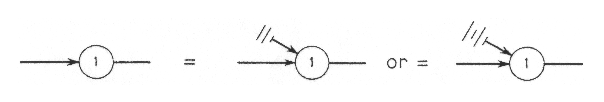
\includegraphics[width=3.4in]{fig_4}
\caption{\label{fig:4}}
\end{figure}

Now the proof can be effected by induction over the number
$p=p(P)$ of symbols used in the definitory expression for $P$
(counting each occurrence of each symbol separately).

If $p(P)=1$, then $P(x_1, \dots, x_n)\equiv x_\nu$ (for one of the
$\nu = 1, \dots, n$). The ``trivial" network which obtains by
breaking off all input lines other than $\nu$, and taking the
input line $\nu$ directly to the output, solves the problem with
$s=0$. Hence $s^*(P)=0$.

If $p(P)>1$, then $P\equiv Q^{-1}$ or $P \equiv QR$ or $P \equiv
Q+R$, where $p(Q)$, $p(R)<p(P)$. For $P\equiv Q^{-1}$ let the box
$\fbox{Q}$ represent a $Q,s'$-network, with $s'=s^*(Q)$. Then the
network shown in Figure~\ref{fig:5} is clearly a $P,s$-network,
with $s=s'+1$. Hence $s^*(P)\leq s^*(Q)+1$. For $P\equiv QR$ or
$Q+R$ let the boxes $\fbox{Q}$, $\fbox{R}$ represent a
$Q,s"$-network and an $R,s"$-network, respectively, with
$s"=\mathrm{Max}(s^*(Q),s^*(R))$. Then the network shown in
Figure~\ref{fig:6} is clearly a $P,s$-network, with $P\equiv QR$
or $Q+R$ for $h=2$ or $1$, respectively, and with $s'=s"+1$. Hence
$s^*(P)\leq \mathrm{Max}(s^*(Q), s^*(R))+1$.

\begin{figure}[t]

\includegraphics[width=3.4in]{fig_5}
\caption{\label{fig:5}}
\end{figure}

\begin{figure}[b]

\includegraphics[width=3.4in]{fig_6}
\caption{\label{fig:6}}
\end{figure}

Combine the above theorem with the fact that every single output
automaton can be equivalently described - apart from its time
delay $s$ - by a polynomial $P$, and that the basic operations
$ab$, $a+b$, $a^{-1}$ of the propositional calculus are
represented (with unit delay) by the basic organs of
Figure~\ref{fig:2}. (For the last one, which represents $ab^{-1}$,
cf. the remark at the beginning of \ref{sec:four1_1}. This
gives:\\

\noindent \textsc{Definition 3:} Two single output automata are
equivalent in the wider sense, if they differ only in their time
delays - but otherwise the same input stimuli produce the same
output stimulus (or non-stimulus) in both.\\

\noindent \textsc{Theorem 2} (Reduction Theorem): Any single
output automaton $r$ is equivalent in the wider sense to a network
of basic organs of Figure~\ref{fig:2}. There exists a (unique)
$s^*=s^*(r)$, such that the latter network exists if and only if
its prescribed time $s$ satisfies $s\geq s^*$.

\subsection{\label{sec:three3}General Logical Considerations}

Now networks of arbitrary single output automata can be replaced
by networks of basic organs of Figure~\ref{fig:2}: It suffices to
replace the unit delay in the former system by $\bar{s}$ unit
delays in the latter, where $\bar{s}$ is the maximum of the
$s^*(r)$ of all the single output automata that occur in multiples
of $\bar{s}$, hence $\geq \bar{s}$, hence $\geq s^*(r)$ for all
$r$ that can occur in this situation, and so the Reduction Theorem
will be applicable throughout.

Thus this system of basic organs is universal: It permits the
construction of essentially equivalent networks to any network
that can be constructed from any system of single output automata.
I.e., no redefinition of the system of basic organs can extend the
logical domain covered by the derived networks.

The general automaton is any network of single output automata in
the above sense. It must be emphasized, that, in particular,
feedbacks, i.e., arrangements of lines which may allow cyclical
stimulation sequences, are allowed. (I.e., configurations like
those shown in Figure~\ref{fig:7}. There will be various,
non-trivial, examples of this later.) The above arguments have
shown, that a limitation of the underlying single output automata
to our original basic organs causes no essential loss of
generality. The question, as to which logical operations can be
equivalently represented (with suitable, but not \textit{a priori}
specified, delays) is nevertheless not without difficulties.

These general automata are, in particular, not immediately
equivalent to all of effectively constructive (intuitionistic)
logics. I.e., given a problem involving (a finite number of)
variables, which can be solved (identically in these variables) by
effective construction, it is not always possible to construct a
general automaton that will produce this solution identically
(i.e., under all conditions). The reason for this is essentially,
that the memory requirements of such a problem may depend on
(actual values assumed by) the variables (i.e., they must be
finite for any specific system of values of the variables, but
they may be unbounded for the totality of all possible systems of
values), while a general automaton in the above sense necessarily
has a fixed memory capacity. I.e., a fixed general automaton can
only handle (identically, i.e., generally) a problem with fixed
(bounded) memory requirements.

We need not go here into the details of this question. Very simple
addenda can be introduced to provide for a (finite but) unlimited
memory capacity. How this can be done has been shown by A. M.
Turing \cite{Turing36}. Turing's analysis \textit{loc. cit.} also
shows, that with such addenda general automata become strictly
equivalent to effectively constructive (intuitionistic) logics.
Our system in its present form (i.e., general automata with
limited memory capacity) is still adequate for the treatment of
all problems with neurological analogies, as our subsequent
examples will show. (Cf. also W. S. McCulloch and W. Pitts
\cite{McCulloch43}.) The exact logical domain that they cover has
been recently characterized by Kleene \cite{Kleene56}. We will
return to some of these questions in \ref{sec:five1}.

\begin{figure}[t]

\includegraphics[width=3.4in]{fig_7}
\caption{\label{fig:7}}
\end{figure}

\section{\label{sec:four}Basic Organs}

\subsection{\label{sec:four1}Reduction of the Basic Components}

\subsubsection{\label{sec:four1_1}The Simplest Reductions} The
previous section makes clear the way in which the elementary
neurons should be interpreted logically. Thus the ones shown in
Figure~\ref{fig:2} respectively represent the logical functions
$ab$, $a+b$, and $ab^{-1}$. In order to get $b^{-1}$, it suffices
to make the $a$-terminal of the third organ, as shown in
Figure~\ref{fig:8}, live. This will be abbreviated in the
following, as shown in Figure~\ref{fig:8}.

\begin{figure}[b]

\includegraphics[width=3.4in]{fig_8}
\caption{\label{fig:8}}
\end{figure}

Now since $ab\equiv ((a^{-1})+(b^{-1}))^{-1}$ and $a+b\equiv
((a^{-1})(b^{-1}))^{-1}$, it is clear that the first organ among
the three basic organs shown in Figure~\ref{fig:2} is equivalent
to a system built of the remaining two organs there, and that the
same is true for the second organ there. Thus the first and second
organs shown in Figure~\ref{fig:2} are respectively equivalent (in
the wider sense) to the two networks shown in Figure~\ref{fig:9}.
This tempts one to consider a new system, in which
$-\circ\bigcirc-$ (viewed as a basic entity in its own right, and
not an abbreviation for a composite, as in Figure~\ref{fig:8}),
and either the first or the second basic organ in
Figure~\ref{fig:2}, are the basic organs. They permit forming the
second or the first basic organ in Figure~\ref{fig:2},
respectively, as shown above, as (composite) networks. The third
basic organ in Figure~\ref{fig:2} is easily seen to be also
equivalent (in the wider sense) to a composite of the above, but,
as was observed at the beginning of \ref{sec:four1_1} the
necessary organ is in any case not this, but $-\circ\bigcirc-$
(cf. also the remarks concerning Figure~\ref{fig:8}),
respectively. Thus either system of new basic organs permits
reconstructing (as composite networks) all the (basic) organs of
the original system. It is true, that these constructs have delays
varying from 1 to 3, but since unit delays, as shown in
Figure~\ref{fig:4}, are available in either new system, all these
delays can be brought up to the value 3. Then a trebling of the
unit delay time obliterates all differences.

\begin{figure}[t]
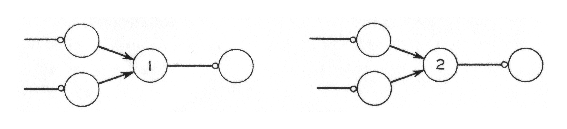
\includegraphics[width=3.4in]{fig_9}
\caption{\label{fig:9}}
\end{figure}

To restate: Instead of the three original basic organs, shown
again in Figure~\ref{fig:10}, we can also (essentially
equivalently) use the two basic organs Nos. one and three or Nos.
two and three in Figure~\ref{fig:10}.

\begin{figure}[b]

\includegraphics[width=3.4in]{fig_10}
\caption{\label{fig:10}}
\end{figure}

\subsubsection{\label{sec:four1_2}The Double Line Trick} This result suggests strongly
that one consider the one remaining combination, too: The two
basic organs Nos. one and two in Figure~\ref{fig:10}, as the basis
of an essentially equivalent system.

One would be inclined to infer that the answer must be negative:
No network built out of the two first basic organs of
Figure~\ref{fig:10} can be equivalent (in the wider sense) to the
last one. Indeed, let us attribute to T and F, i.e., to the
stimulated or non-stimulated state of a line, respectively, the
``truth values" $\underline{1}$ or $\underline{0}$, respectively.
Keeping the ordering $\underline{0}<\underline{1}$ in mind, the
state of the output is a monotone non-decreasing function of the
states of the inputs for both basic organs Nos. one and two in
Figure~\ref{fig:10}, and hence for all networks built from these
organs exclusively as well. This, however, is not the case for the
last organ of Figure~\ref{fig:10} (nor for the last organ of
Figure~\ref{fig:2}), irrespectively of delays.

Nevertheless a slight change of the underlying definitions permits
one to circumvent this difficulty, and to get rid of the negation
(the last organ of Figure~\ref{fig:10}) entirely. The device which
effects this is of additional methodological interest, because it
may be regarded as the prototype of one that we will use later on
in a more complicated situation. The trick in question is to
represent propositions on a double line instead of a single one.
One assumes that of the two lines, at all times precisely one is
stimulated. Thus there will always be two possible states of the
line pair: The first line stimulated, the second non-stimulated;
and the second line stimulated, the first non-stimulated. We let
one of these states correspond to the stimulated single line of
the original system - that is, to a true proposition - and the
other state to the unstimulated single line - that is, to a false
proposition. Then the three fundamental Boolean operations can be
represented by the three first schemes shown in
Figure~\ref{fig:11}. (The last scheme shown in Figure~\ref{fig:11}
relates to the original system in Figure~\ref{fig:2}.)

\begin{figure}
\includegraphics[width=3.4in]{fig_11}
\caption{\label{fig:11}}
\end{figure}

In these diagrams, a true proposition corresponds to $1$
stimulated, $2$ unstimulated, while a false proposition
corresponds to $1$ unstimulated, $2$ stimulated. The networks of
Figure~\ref{fig:11}, with the exception of the third one, have
also the correct delays: Unit delay. The third one has zero delay,
but whenever this is not wanted, it can be replaced by unit delay,
by replacing the third network by the fourth one, making its
$a1$-line live, its $a2$-line grounded, and then writing $a$ for
its $b$.

Summing up: Any two of the three (single delay) organs of
Figure~\ref{fig:10} - which may simply be designated $ab$, $a+b$,
$a^{-1}$ - can be stipulated to be the basic organs, and yield a
system that is essentially equivalent to the original one.

\subsubsection{\label{sec:four2_1}The Sheffer Stroke} It is even
possible to reduce the number of basic organs to one, although it
cannot be done with any of the three organs enumerated above. We
will, however, introduce two new organs, either of which suffices
by itself.

The first universal organ corresponds to the well-known ``Sheffer
stroke" function. Its use in this context was suggested by K. A.
Brueckner and G. Gell-Mann. In symbols, it can be represented (and
abbreviated) as shown on Figure~\ref{fig:12}. The three
fundamental Boolean operations can now be performed as shown in
Figure~\ref{fig:13}.

\begin{figure}[b]
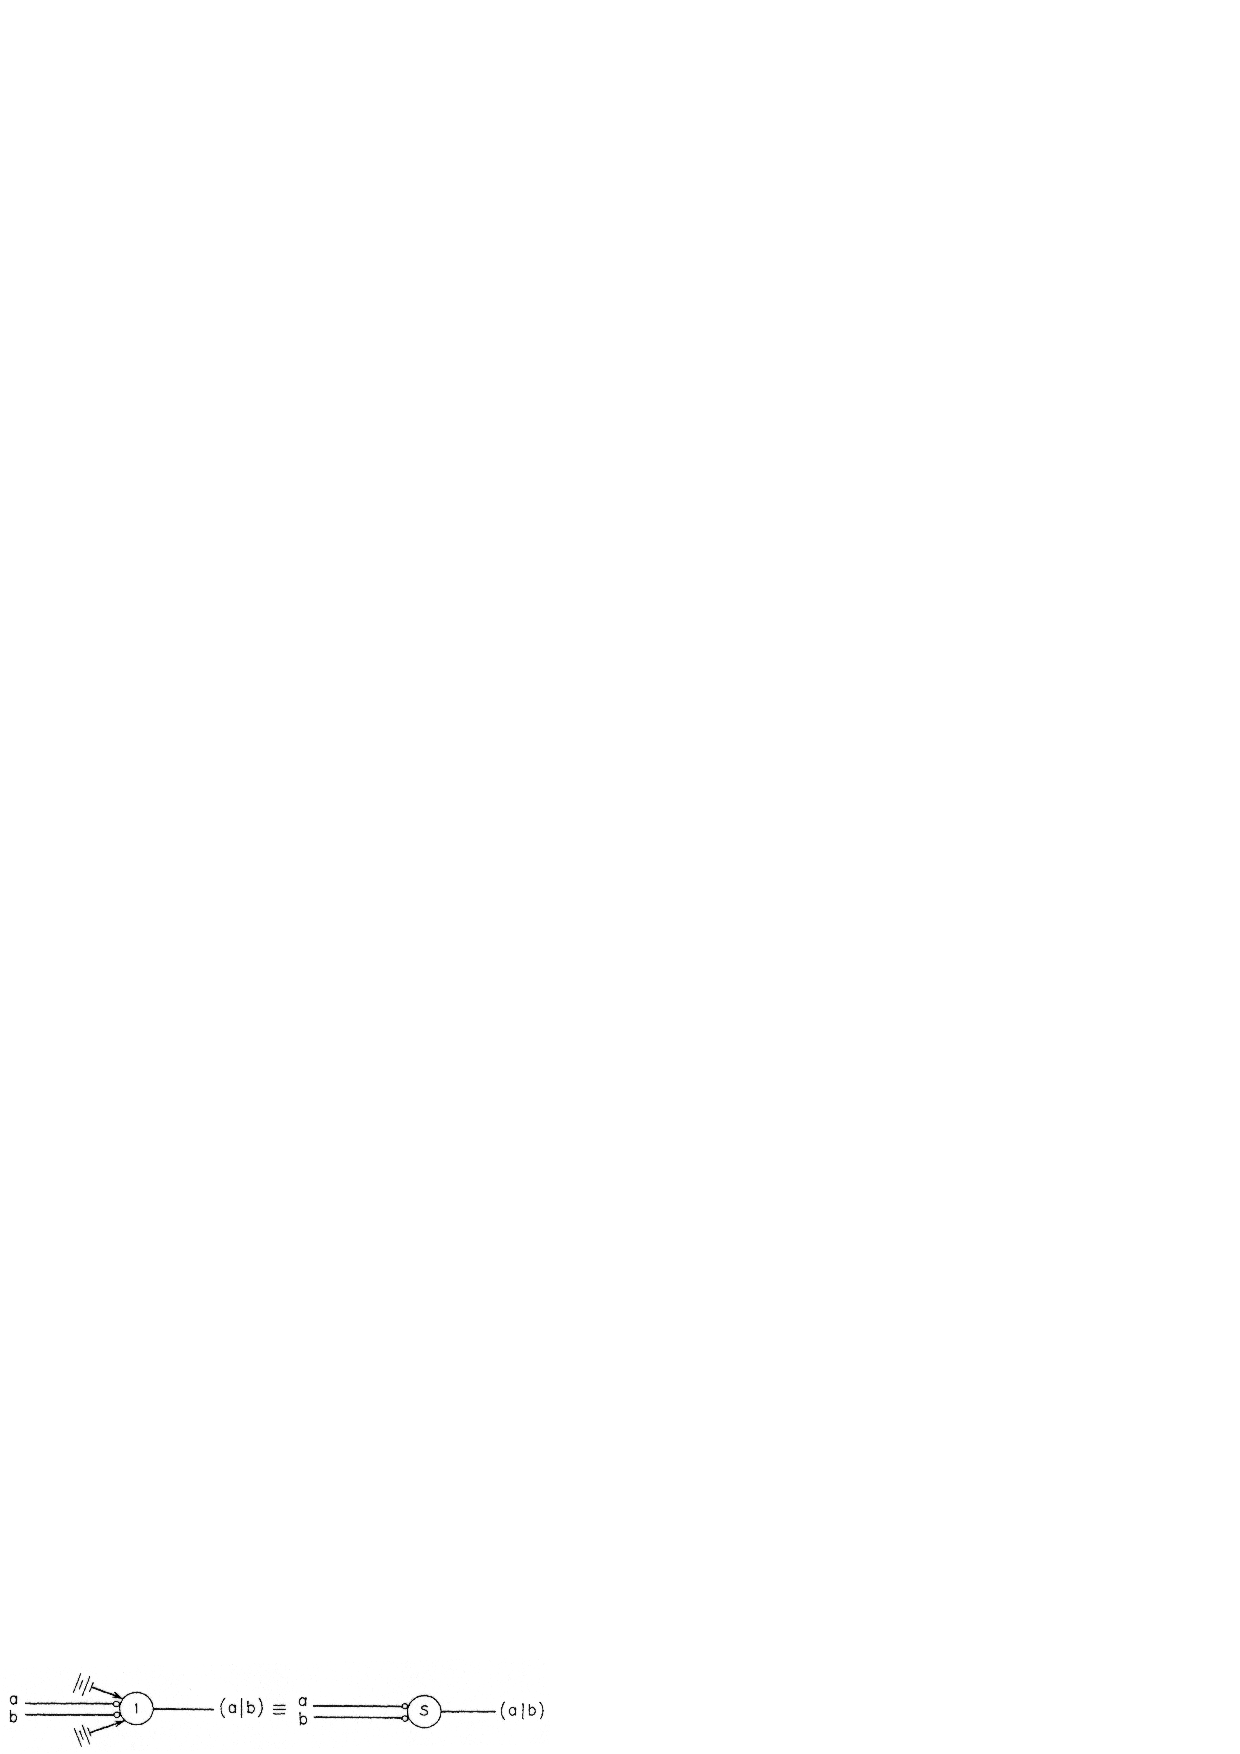
\includegraphics[width=3.4in]{fig_12}
\caption{\label{fig:12}$(a|b)\equiv (ab)^{-1}$}
\end{figure}

\begin{figure}[t]
\includegraphics[width=3.4in]{fig_13}
\caption{\label{fig:13}}
\end{figure}

The delays are 2, 2, 1, respectively, and in this case the
complication caused by these delay-relationships is essential.
Indeed, the output of the Sheffer-stroke is an antimonotone
function of its inputs. Hence in every network derived from it,
even-delay outputs will be monotone functions of its inputs, and
odd-delay outputs will be antimonotone ones. Now $ab$ and $a+b$
are not antimonotone, and $ab^{-1}$ and $a^{-1}$ are not monotone.
Hence no delay-value can simultaneously accommodate in this set up
one of the two first organs and one of the two last organs.

The difficulty can, however, be overcome as follows: $ab$ and
$a+b$ are represented in Figure~\ref{fig:13}, both with the same
delay, namely 2. Hence our earlier result (in \ref{sec:four1_2}),
securing the adequacy of the system of the two basic organs $ab$
and $a+b$ applies: Doubling the unit delay time reduces the
present set up (Sheffer stroke only!) to the one referred to
above.

\subsubsection{\label{sec:four2_2}The Majority Organ} The second
universal organ is the ``majority organ". In symbols, it is shown
(and alternatively designated) in Figure~\ref{fig:14}. To get
conjunction and disjunction, is a simple matter, as shown in
Figure~\ref{fig:15}. Both delays are $1$. Thus $ab$ and $a+b$
(according to Figure~\ref{fig:10}) are correctly represented, and
the new system (majority organ only!) is adequate because the
system based on those two organs is known to be adequate (cf.
\ref{sec:four1_2}).

\begin{figure}[b]
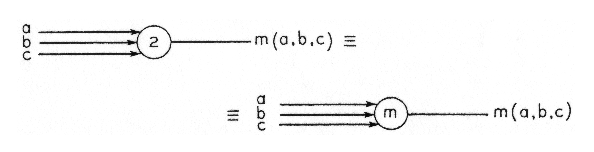
\includegraphics[width=3.4in]{fig_14}
\caption{\label{fig:14}$m(a,b,c)\equiv ab+ac+bc\equiv
(a+b)(a+c)(b+c)$}
\end{figure}

\begin{figure}
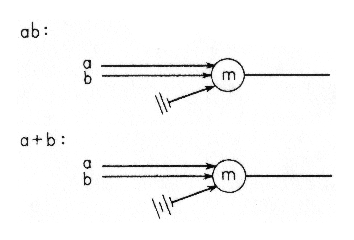
\includegraphics[width=3.2in]{fig_15}
\caption{\label{fig:15}}
\end{figure}

\section{\label{sec:five}Logics and Information}

\subsection{\label{sec:five1}Intuitionistic Logics}

All of the examples which have been described in the last two
sections have had a certain property in common; in each, a
stimulus of one of the inputs at the left could be traced through
the machine until at a certain time later it came out as a
stimulus of the output on the right. To be specific, no pulse
could ever return to a neuron through which it had once passed. A
system with this property is called circle-free by W. S. McCulloch
and W. Pitts \cite{McCulloch43}. While the theory of circle-free
machines is attractive because of its simplicity, it is not hard
to see that these machines are very limited in their scope.

When the assumption of no circles in the network is dropped, the
situation is radically altered. In this far more complicated case,
the output of the machine at any time may depend on the state of
the inputs in the indefinitely remote past. For example, the
simplest kind of cyclic circuit, as shown in Figure~\ref{fig:16},
is a kind of memory machine. Once this organ has been stimulated
by $a$, it remains stimulated and sends forth a pulse in $b$ at
all times thereafter. With more complicated networks, we can
construct machines which will count, which will do simple
arithmetic, and which will even perform certain unlimited
inductive processes. Some of these will be illustrated by examples
in \ref{sec:six}. The use of cycles or feedback in automata
extends the logic of constructible machines to a large portion of
intuitionistic logic. Not all of the intuitionistic logic is so
obtained, however, since these machines are limited by their fixed
size. (For this, and for the remainer of this chapter cf. also the
remarks at he end of \ref{sec:three3}.) Yet, if our automata are
furnished with an unlimited memory - for example, an infinite
tape, and scanners connected to afferent organs, along with
suitable efferent organs to perform motor operations and/or print
on the tape - the logic of constructible machines becomes
precisely equivalent to intuitionistic logic (see A. M. Turing
\cite{Turing36}). In particular, all numbers computable in the
sense of Turing can be computed by some such network.

\begin{figure}[b]

\includegraphics[width=3in]{fig_16}
\caption{\label{fig:16}}
\end{figure}

\subsection{\label{sec:five2}Information}

\subsubsection{\label{sec:five2_1}General Observations} Our
considerations deal with varying situations, each of which
contains a certain amount of information. It is desirable to have
a means of measuring that amount. In most cases of importance,
this is possible. Suppose an event is one selected from a finite
set of possible events. Then the number of possible events can be
regarded as a measure of the information content of knowing which
event occurred, provided all events are \textit{a priori} equally
possible. However, instead of using the number $n$ of possible
events as the measure of information, it is advantageous to use a
certain function of $n$, namely the logarithm. This step can be
(heuristically) justified as follows: If two physical systems I
and II represent $n$ and $m$ (\textit{a priori} equally probable)
alternatives, respectively, then union $\mathrm{I}+\mathrm{II}$
represents $nm$ such alternatives. Now it is desirable that the
(numerical) measure of information be (numerically) additive under
this (substantially) additive composition
$\mathrm{I}+\mathrm{II}$. Hence some function $f(n)$ should be
used instead of $n$, such that

\begin{equation}
f(nm)=f(n) + f(m)~. \label{eq:3}
\end{equation}

\noindent In addition, for $n>m$ $\mathrm{I}$ represents more
information than $\mathrm{II}$, hence it is reasonable to require

\begin{equation}
n>m ~~ \mathrm{implies} ~~ f(n) > f(m)~. \label{eq:4}
\end{equation}

\noindent Note, that $f(n)$ is defined for $n=1,2,\ldots$ only.
From Eqs.~\ref{eq:3} and \ref{eq:4} one concludes easily, that

\begin{equation}
f(n)\equiv C\ln{n}\label{eq:5}
\end{equation}

\noindent for some constant $C>0$. (Since $f(n)$ is defined for
$n=1,2,\ldots$ only, Eq.~\ref{eq:3} alone does not imply this,
even not with a constant $C \gtreqqless 0$ !) Next, it is
conventional to let the minimum non-vanishing amount of
information, i.e., that which corresponds to $n=2$, be the unit of
information - the ``bit". This means that $f(2)=1$, i.e.,
$C=1/\ln{2}$, and so

\begin{equation}
f(n)\equiv \log_{2}{n}~.\label{eq:6}
\end{equation}

\noindent This concept of information was successively developed
by several authors in the late 1920's and early 1930's, and
finally integrated into a broader system by C. E. Shannon
\cite{Shannon48}.

\subsubsection{\label{sec:five2_2}Examples} The following simple
examples give some illustration: The outcome of the flip of a coin
is one bit. That of the roll of a die is $\log_{2}{6}=2.5$ bits. A
decimal digit represents $\log_{2}{26}=4.7$ bits, a single
character from a 44-key, 2-setting typewriter represents
$\log_{2}{44\times 2}=6.5$ bits. (In all these we assume, for the
sake of the argument, although actually unrealistically, \textit{a
priori} equal probability of all possible choices.) It follows
that any line or nerve fibre which can be classified as either
stimulated or non-stimulated carries precisely one bit of
information, while a bundle of $n$ such lines can communicate $n$
bits. It is important to observe that this definition is possible
only on the assumption that a background of \textit{a priori}
knowledge exists, namely, the knowledge of a system of \textit{a
priori} equally probable events.

This definition can be generalized to the case where the possible
events are not all equally probable. Suppose the events are known
to have probabilities $p_1, p_2, \ldots, p_n$. Then the
information contained in the knowledge of which of these events
actually occurs, is defined to be

\begin{equation}
H =
-\sum_{i=1}^{n}{p_i\log_{2}{p_i}}~~(\mathrm{bits})~.\label{eq:7}
\end{equation}

\noindent In case $p_1=p_2=\ldots = p_n = 1/n$, this definition is
the same as the previous one. This result, too, was obtained by C.
E. Shannon \cite{Shannon48}, although it is implicit in the
earlier work of L. Szilard \cite{Szilard29}.

An important observation about this definition is that it bears
close resemblance to the statistical definition of the entropy of
a thermodynamical system. If the possible events are just the
known possible states of the system with their corresponding
probabilities, then the two definitions are identical. Pursuing
this, one can construct a mathematical theory of the communication
of information patterned after statistical mechanics. (See L.
Szilard \cite{Szilard29} and C. E. Shannon \cite{Shannon48}.) That
information theory should thus reveal itself as an essentially
thermodynamical discipline, is not at all surprising: The
closeness and the nature of the connection between information and
entropy in inherent in L. Boltzman's classical definition of
entropy (apart from a constant, dimensional factor) as the
logarithm of the ``configuration number." The ``configuration
number" is the number of \textit{a priori} equally probable states
that are compatible with the macroscopic description of the state
- i.e., it corresponds to the amount of (microscopic) information
that is missing in the (macroscopic) description.

\section{\label{sec:six}Typical Synthesis of Automata}

\subsection{\label{sec:six1}The Memory Unit}

One of the best ways to become familiar with the ideas which have
been introduced, is to study some concrete examples of simple
networks. This section is devoted to a consideration of a few of
them.

The first example will be constructed with the help of the three
basic organs of Figure~\ref{fig:10}. It is shown in
Figure~\ref{fig:18}. It is a slight refinement of the primitive
memory network of Figure~\ref{fig:16}.

\begin{figure}

\includegraphics[width=3.2in]{fig_17}
\caption{\label{fig:17}}
\end{figure}

This network has two inputs $a$ and $b$ and one output $x$. At
time $t$, $x$ is stimulated if and only if $a$ has been stimulated
at an earlier time, and no stimulation of $b$ has occurred since
then. Roughly speaking, the machine remembers whether $a$ or $b$
was the last input to be stimulated. Thus $x$ is stimulated, if it
has been stimulated immediately before - to be designated by $x'$
- or if $a$ has been stimulated immediately before, but $b$ has
not been stimulated immediately before. This is expressed by the
formula $x=(x'+a)b^{-1}$, i.e., by the network shown in
Figure~\ref{fig:17}. Now $x$ should be fed back into $x'$ (since
$x'$ is the immediately preceding state of $x$). This gives the
network shown in Figure~\ref{fig:18}, where this branch of $x$ is
designated by $y$. However, the delay of the first network is 2,
hence the second network's memory extends over past events that
lie an even number of time (delay) units back. I.e., the output
$x$ is stimulated if and only if $a$ has been stimulated at an
earlier time, an even number of units before, and no stimulation
of $b$ has occurred since then, also an even number of units
before. Enumerating the time units by an integer $t$, it is thus
seen, that this network represents a separate memory for even and
for odd $t$. For each case it is a simple ``off-on", i.e., one
bit, memory. Thus it is in its entirety a two bit memory.

\begin{figure}[t]

\includegraphics[width=3.4in]{fig_18}
\caption{\label{fig:18}}
\end{figure}

\subsection{\label{sec:six2}Scalars}

In the examples that follow, free use will be made of the general
family of basic organs considered in \ref{sec:two3}, at least for
all $\phi = x_h$ (cf. Eq.~\ref{eq:2}) there). The reduction thence
to elementary organs in the original sense is secured by the
Reduction Theorem in \ref{sec:three2}, and in the subsequently
developed interpretations, according to section~\ref{sec:four}, by
our considerations there. It is therefore unnecessary to concern
ourselves here with these reductions.

The second example is a machine which counts input stimuli by
two's. It will be called a ``scalar by two". Its diagram is shown
in Figure~\ref{fig:19}.

\begin{figure}[b]
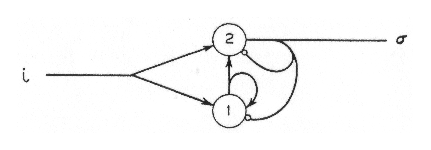
\includegraphics[width=3.4in]{fig_19}
\caption{\label{fig:19}}
\end{figure}

By adding another input, the repressor, the above mechanism can be
turned off at will. The diagram becomes as shown in
Figure~\ref{fig:20}. The result will be called a ``scalar by two"
with a repressor and denoted as indicated by  Figure~\ref{fig:20}.

\begin{figure}[b]
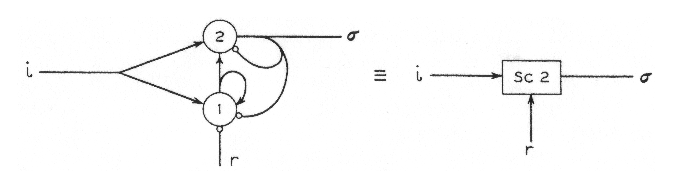
\includegraphics[width=3.4in]{fig_20}
\caption{\label{fig:20}}
\end{figure}

In order to obtain larger counts, the ``scalar by two" networks
can be hooked in series. Thus a ``scalar by $2^n$" is shown in
Figure~\ref{fig:21}. The use of the repressor is of course
optional here. ``Scalars by $m$", where $m$ is not necessarily of
the form $2^n$, can also be constructed with little difficulty,
but we will not go into this here.

\begin{figure}[t]
\includegraphics[width=3.4in]{fig_21}
\caption{\label{fig:21}}
\end{figure}

\subsection{\label{sec:six3}Learning}

Using these ``scalars by $2^n$" (i.e., n-stage counters), it is
possible to construct the following sort of ``learning device".
This network has two inputs $a$ and $b$. It is designed to learn
that whenever $a$ is stimulated, then, in the next instant, $b$
will be stimulated. If this occurs 256 times (not necessarily
consecutively and possibly with many exceptions to the rule), the
machine learns to anticipate a pulse from $b$ one unit of time
after $a$ has been active, and expresses this by being stimulated
at its $b$ output after every stimulation of $a$. The diagram is
shown in Figure~\ref{fig:22}. (The ``expression" described above
will be made effective in the desired sense by the network of
Figure~\ref{fig:24}, cf. its discussion below).

This is clearly learning in the crudest and most inefficient way,
only. With some effort, it is possible to refine the machine so
that, first, it will learn only if it receives  no
counter-instances of the pattern ``$b$ follows $a$" during the
time when it is collecting these 256 instances; and, second,
having once learned, the machine can unlearn by the occurrences of
64 counter-examples to ``$b$ follows $a$" if no (positive)
instances of this pattern interrupt the (negative) series.
Otherwise, the behavior is as before. The diagram is shown in
Figure~\ref{fig:23}. To make this learning effective, one has to
use $x$ to gate $a$ so as to replace $b$ at its normal functions.
Let these be represented by an output $c$. Then this process is
mediated by the network shown in Figure~\ref{fig:24}. This network
must then be attached to the lines $a,b$ and to the output $x$ of
the preceding network (according to Figures~\ref{fig:22},
\ref{fig:23}).

\begin{figure}[b]
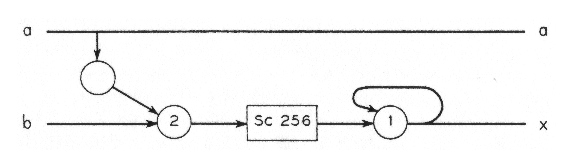
\includegraphics[width=3.4in]{fig_22}
\caption{\label{fig:22}}
\end{figure}

\begin{figure}[t]
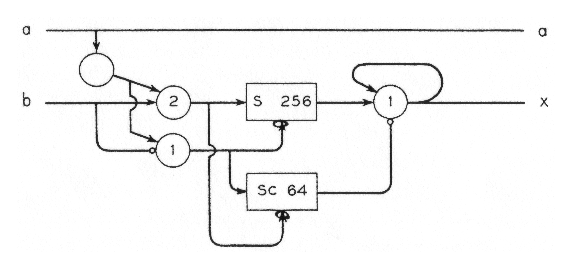
\includegraphics[width=3.55in]{fig_23}
\caption{\label{fig:23}}
\end{figure}

\begin{figure}[b]
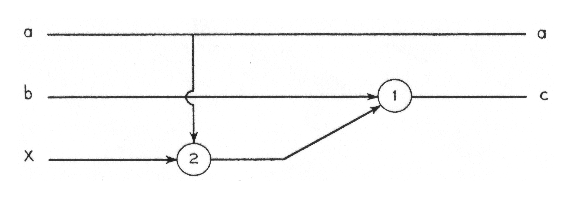
\includegraphics[width=3.4in]{fig_24}
\caption{\label{fig:24}}
\end{figure}

\section{\label{sec:seven}The Role of Error}

\subsection{\label{sec:seven1}Exemplification with the Help of the Memory Unit}

In all the previous considerations, it has been assumed that the
basic components were faultless in their performance. This
assumption is clearly not a very realistic one. Mechanical devices
as well as electrical ones are statistically subject to failure,
and the same is probably true for animal neurons too. Hence it is
desirable to find a closer approximation to reality as a basis for
our constructions, and to study this revised situation. The
simplest assumption concerning errors is this: With every basic
organ is associated a positive number $\epsilon$ such that in any
operation, the organ will fail to function correctly with the
(precise) probability $\epsilon$. This malfunctioning is assumed
to occur statistically independently of the general state of the
network and of the occurrence of other malfunctions. A more
general assumption, which is a good deal more realistic, is this:
The malfunctions are statistically dependent on the general state
of the network and on each other. In any particular state,
however, a malfunction of the basic organ in question has a
probability of malfunctioning which is $\leq \epsilon$. For the
present occasion, we make the first (narrower and simpler)
assumption, and that with a single $\epsilon$: Every neuron has
statistically independently of all else exactly the probability
$\epsilon$ of misfiring. Evidently, it might as well be supposed
$\epsilon \leq 1/2$, since an organ which consistently misbehaves
with a probability $> 1/2$, is just behaving with the negative of
its attributed function, and a (complementary) probability of
error $< 1/2$. Indeed, if the organ is thus redefined as its own
opposite, its $\epsilon$ ($> 1/2$) goes then over into
$1-\epsilon$ ($< 1/2$). In practice it will be found necessary to
have $\epsilon$ a rather small number, and one of the objectives
of this investigation is to find the limits of this smallness,
such that useful results can still be achieved.

It is important to emphasize, that the difficulty introduced by
allowing error is not so much that incorrect information will be
obtained, but rather that irrelevant results will be produced. As
a simple example, consider the memory organ of
Figure~\ref{fig:16}. Once stimulated, this network should continue
to emit pulses at all later times; but suppose it has the
probability $\epsilon$ of making an error. Suppose the organ
receives a stimulation at time $t$ and no later ones. Let the
probability that the organ is still excited after $s$ cycles be
denoted $\rho_s$. Then the recursion formula

\begin{equation*}
\rho_{s+1}=(1-\epsilon)\rho_s+\epsilon(1-\rho_s)
\end{equation*}

\noindent is clearly satisfied. This can be written

\begin{equation*}
\rho_{s+1}-1/2=(1-2\epsilon)(\rho_s-1/2)
\end{equation*}

\noindent and so

\begin{eqnarray}
\rho_s-1/2 & = & (1-2\epsilon)^s(\rho_0-1/2)\\
           &   & \sim \mathrm{e}^{-2\epsilon s}(\rho_0-1/2) \label{eq:8}
\end{eqnarray}

\noindent for small $\epsilon$. The quantity $\rho_s-1/2$ can be
taken as a rough measure of the amount of discrimination in the
system after the $s$-th cycle. According to the above formula,
$\rho_s\rightarrow1/2$ as $s\rightarrow \infty$ - a fact which is
expressed by saying that, after a long time, the memory content of
the machine disappears, since it tends to equal likelihood of
being right or wrong, i.e., to irrelevancy.

\subsection{\label{sec:seven2}The General Definition}

This example is typical of many. In a complicated network, with
long stimulus-response chains, the probability of errors in the
basic organs makes the response of the final outputs unreliable,
i.e., irrelevant, unless some control mechanism prevents the
accumulation of these basic errors. We will consider two aspects
of this problem. Let the data be these: The function which the
automaton is to perform is given; a basic organ is given (Sheffer
stroke, for example); a number $\epsilon$ ($<1/2$), which is the
probability of malfunctioning of this basic organ, is prescribed.
The first question is: Given $\delta>0$, can a corresponding
automaton be constructed from the given organs, which will perform
the desired function and will commit an error (in the final
result, i.e., output) with probability $\leq\delta$? How small can
$\delta$ be prescribed? The second question is: Are there other
ways to interpret the problem which will allow us to improve the
accuracy of the result?

\subsection{\label{sec:seven3}An Apparent Limitation}

In partial answer to the first question, we notice now that
$\delta$, the prescribed maximum allowable (final) error of the
machine, must not be less than $\epsilon$. For any output of the
automaton is the immediate result of the operation of a single
final neuron and the reliability of the whole system cannot be
better than the reliability of this last neuron.

\subsection{\label{sec:seven4}The Multiple Line Trick}

In answer to the second question, a method will be analyzed by
which this threshold restriction $\delta\geq\epsilon$ can be
removed. In fact we will be able to prescribe $\delta$ arbitrarily
small (for suitable, but fixed, $\epsilon$). The trick consists in
carrying all the messages simultaneously on a bundle of $N$ lines
($N$ is a large integer) instead of just a single or double strand
as in the automata described up to now. An automaton would then be
represented by a black box with several bundles of inputs and
outputs, as shown Figure~\ref{fig:25}. Instead of requiring that
all or none of the lines of the bundle be stimulated, a certain
critical (or fiduciary level) $\Delta$ is set: $0<\Delta<1/2$. The
stimulation of $\geq(1-\Delta)N$ lines of a bundle is interpreted
as a positive state of the bundle. The stimulation of $\leq\Delta
N$ lines is considered as a negative state. All levels of
stimulation between these values are intermediate or undecided. It
will be shown that by suitably constructing the automaton, the
number of lines deviating from the ``correctly functioning"
majorities of their bundles can be kept at or below or critical
level $\Delta N$ (with arbitrary high probability). Such a system
of construction is referred to as ``multiplexing". Before turning
to the multiplexed automata, however, it is well to consider the
ways in which error can be controlled in out customary single line
networks.

\begin{figure}

\includegraphics[width=3in]{fig_25}
\caption{\label{fig:25}Each group $\underline{\equiv}$ represents
a bundle of $N$ lines.}
\end{figure}

\section{\label{sec:eight}Control of Error in Single Line Automata}

\subsection{\label{sec:eight1}The Simplified Probability Assumption}

In \ref{sec:seven3} it was indicated that when dealing with an
automaton in which messages are carried on a single (or even a
double) line, and in which the components have a definite
probability $\epsilon$ of making an error, there is a lower bound
to the accuracy of the operation of machine. It will now be shown
that it is nevertheless possible to keep the accuracy within
reasonable bounds by suitably designing the network. For the sake
of simplicity only circle-free automata (cf. \ref{sec:five1}) will
be considered in this section, although the conclusions could be
extended, with proper safeguards, to all automata. Of the various
essentially equivalent systems of basic organs (cf.
section~\ref{sec:four}) it is, in the present instance, most
convenient to select the majority organ, which is shown in
Figure~\ref{fig:14}, as the basic organ for our networks. The
number $\epsilon$ ($0<\epsilon<1/2$) will denote the probability
each majority organ has for malfunctioning.

\subsection{\label{sec:eight2}The Majority Organ}

We first investigate upper bounds for the probability of errors as
impulses pass through a single majority organ of a network. Three
lines constitute the inputs of the majority organ. They come from
other organs or are external inputs of the network. Let $\eta_1$,
$\eta_2$, $\eta_3$ be three numbers ($0<\eta_1\leq 1$), which are
respectively upper bounds for the probabilities that these lines
will be carrying the wrong impulses. Then $\epsilon + \eta_1 +
\eta_2 + \eta_3$ is an upper bound for the probability that the
output line of the majority organ will act improperly. This upper
bound is valid in all cases. Under proper circumstances it can be
improved. In particular, assume: (i) The probabilities of errors
in the inputs lines are independent, (ii) under proper functioning
of the network, these lines should always be in the same state of
excitation (either all stimulated, or all unstimulated). In this
latter case

\begin{equation*}
\theta=\eta_1\eta_2+\eta_1\eta_3+\eta_2\eta_3-2\eta_1\eta_2\eta_3
\end{equation*}

\noindent is an upper bound for at least two of the input lines
carrying the wrong impulses, and thence

\begin{equation*}
\epsilon'=(1-\epsilon)\theta+\epsilon(1-\theta)=\epsilon+(1-2\epsilon)\theta
\end{equation*}

\noindent is a smaller upper bound for the probability of failure
in the output line. If all $\eta_1\leq\eta$, then $\epsilon+3\eta$
is a general upper bound, and
$\epsilon+(1-2\epsilon)(3\eta^2-2\eta^3)\leq \epsilon+3\eta^2$ is
an upper bound for the special case. Thus it appears that in the
general case each operation of the automaton increases the
probability of error, since $\epsilon+3\eta>\eta$, so that if the
serial depth of the machine (or rather of the process to be
performed) is very great, it will be impractical or impossible to
obtain any kind of accuracy. In the special case, on the other
hand, this is not necessarily so - $\epsilon+3\eta^2<\eta$ is
possible. Hence, the chance of keeping the error under control
lies in maintaining the conditions of the special case throughout
the construction. We will now exhibit a method which achieves
this.

\subsection{\label{sec:eight3}Synthesis of Automata}

\subsubsection{\label{sec:eight3_1}The Heuristic Argument} The
basic idea in this procedure is very simple. Instead of running
the incoming data into a single machine, the same information is
simultaneously fed into a number of identical machines, and the
result that comes out of a majority of these machines is assumed
to be true. It must be shown that this technique can really be
used to control error.

Denote by $\mathcal{O}$ the given network (assume two outputs in
the specific instance picture in Figure~\ref{fig:26}). Construct
$\mathcal{O}$ in triplicate, labelling the copies $\mathcal{O}^1$,
$\mathcal{O}^2$, $\mathcal{O}^3$ respectively. Consider the system
shown in Figure~\ref{fig:26}.

\begin{figure}

\includegraphics[width=3.4in]{fig_26}
\caption{\label{fig:26}}
\end{figure}

For each of the final majority organs the conditions of the
special case considered above obtain. Consequently, if $\eta$ is
an upper bound for the probability of error at any output of the
original network $\mathcal{O}$, then

\begin{equation}
\eta^*=\epsilon+(1-2\epsilon)(3\eta^2-2\eta^3)\equiv
f_\epsilon(\eta) \label{eq:9}
\end{equation}

\noindent is an upper bound for the probability of error at any
output of the new network $\mathcal{O}^*$. The graph is the curve
$\eta^*=f_\epsilon(\eta)$, shown in Figure~\ref{fig:27}.

Consider the intersections of the curve with the diagonal
$\eta^*=\eta$: First, $\eta=1/2$ is at any rate such an
intersection. Dividing $\eta-f_\epsilon(\eta)$ by $\eta-1/2$ gives
$2((1-2\epsilon)\eta^2-(1-2\epsilon)\eta+\epsilon)$, hence the
other intersections are the roots of
$(1-2\epsilon)\eta^2-(1-2\epsilon)\eta+\epsilon=0$, i.e.,

\begin{equation*}
\eta = \frac{1}{2}\left(1 \pm
\sqrt{\frac{1-6\epsilon}{1-2\epsilon}}\right)
\end{equation*}

\noindent I.e., for $\epsilon\geq1/6$ they do not exist (being
complex (for ($\epsilon>1/6$) or $=1/2$ (for $\epsilon=1/6$));
while for $\epsilon<1/6$ they are $\eta=\eta_0$, $1-\eta_0$, where

\begin{equation}
\eta_0=\frac{1}{2}\left(1-\sqrt{\frac{1-6\epsilon}{1-2\epsilon}}\right)=\epsilon+3\epsilon^2+\ldots
\label{eq:10}
\end{equation}

\noindent For $\eta=0$; $\eta^*=\epsilon>\eta$. This, and the
monotony and continuity of $\eta^*=f_\epsilon(\eta)$ therefore
imply:\\

\underline{First case, $\epsilon\geq1/6$}:\\
\indent~~~$0\leq\eta<1/2 \Rightarrow \eta<\eta^*<1/2$;\\
\indent ~~~$1/2<\eta\leq1 \Rightarrow 1/2<\eta^*<\eta$.\\\\
\indent \underline{Second case, $\epsilon<1/6$}:\\
\indent ~~~$0\leq\eta<\eta_0 \Rightarrow \eta<\eta^*<\eta_0$:\\
\indent ~~~$\eta_0<\eta<1/2 \Rightarrow \eta_0<\eta^*<\eta$;\\
\indent ~~~$1/2<\eta<1-\eta_0 \Rightarrow \eta<\eta^*<1-\eta_0$;\\
\indent ~~~$1-\eta_0<\eta<1 \Rightarrow 1-\eta_0<\eta^*<\eta$.\\

Now we must expect numerous successive occurrences of the
situation under consideration, if it is to be used as a basic
procedure. Hence the iterative behavior of the operation
$\eta\rightarrow\eta^*=f_\epsilon(\eta)$ is relevant. Now it is
clear from the above, that in the first case the successive
iterates of the process in question always converge to 1/2, no
matter what the original $\eta$; while in the second case these
iterates converge to $\eta_0$ if the original $\eta<1/2$, and to
$1-\eta_0$ if the original $\eta>1/2$.

In other words: In the first case no error level other than
$\eta\sim1/2$ can maintain itself in the long run. I.e., the
process asymptotically degenerates to total irrelevance, like the
one discussed in \ref{sec:seven1}. In the second case the
error-levels $\eta\sim\eta_0$ and $\eta\sim1-\eta_0$ will not only
maintain themselves in the long run, but they represent the
asymptotic behavior for any original $\eta<1/2$ or $\eta>1/2$,
respectively.

These arguments, although heuristic, make it clear that the second
case alone can be used for the desired error-level control. I.e.,
we must require $\epsilon<1/6$, i.e., the error-level for a single
basic organ function must be less than $\sim 16 \%$. The stable,
ultimate error-level should then be $\eta_0$ (we postulate, of
course, that the start be made with an error-level $\eta<1/2$).
$\eta_0$ is small if $\epsilon$ is, hence $\epsilon$ must be
small, and so

\begin{equation}
\eta_0=\epsilon+3\epsilon^2+\ldots \label{eq:11}
\end{equation}

\noindent This would therefore give an ultimate error-level of
$\sim 10 \%$ (i.e., $\eta_0 \sim 0.1$) for a single basic organ
function error-level of $\sim 8 \%$ (i.e. $\epsilon\sim 0.08$).

\begin{figure}
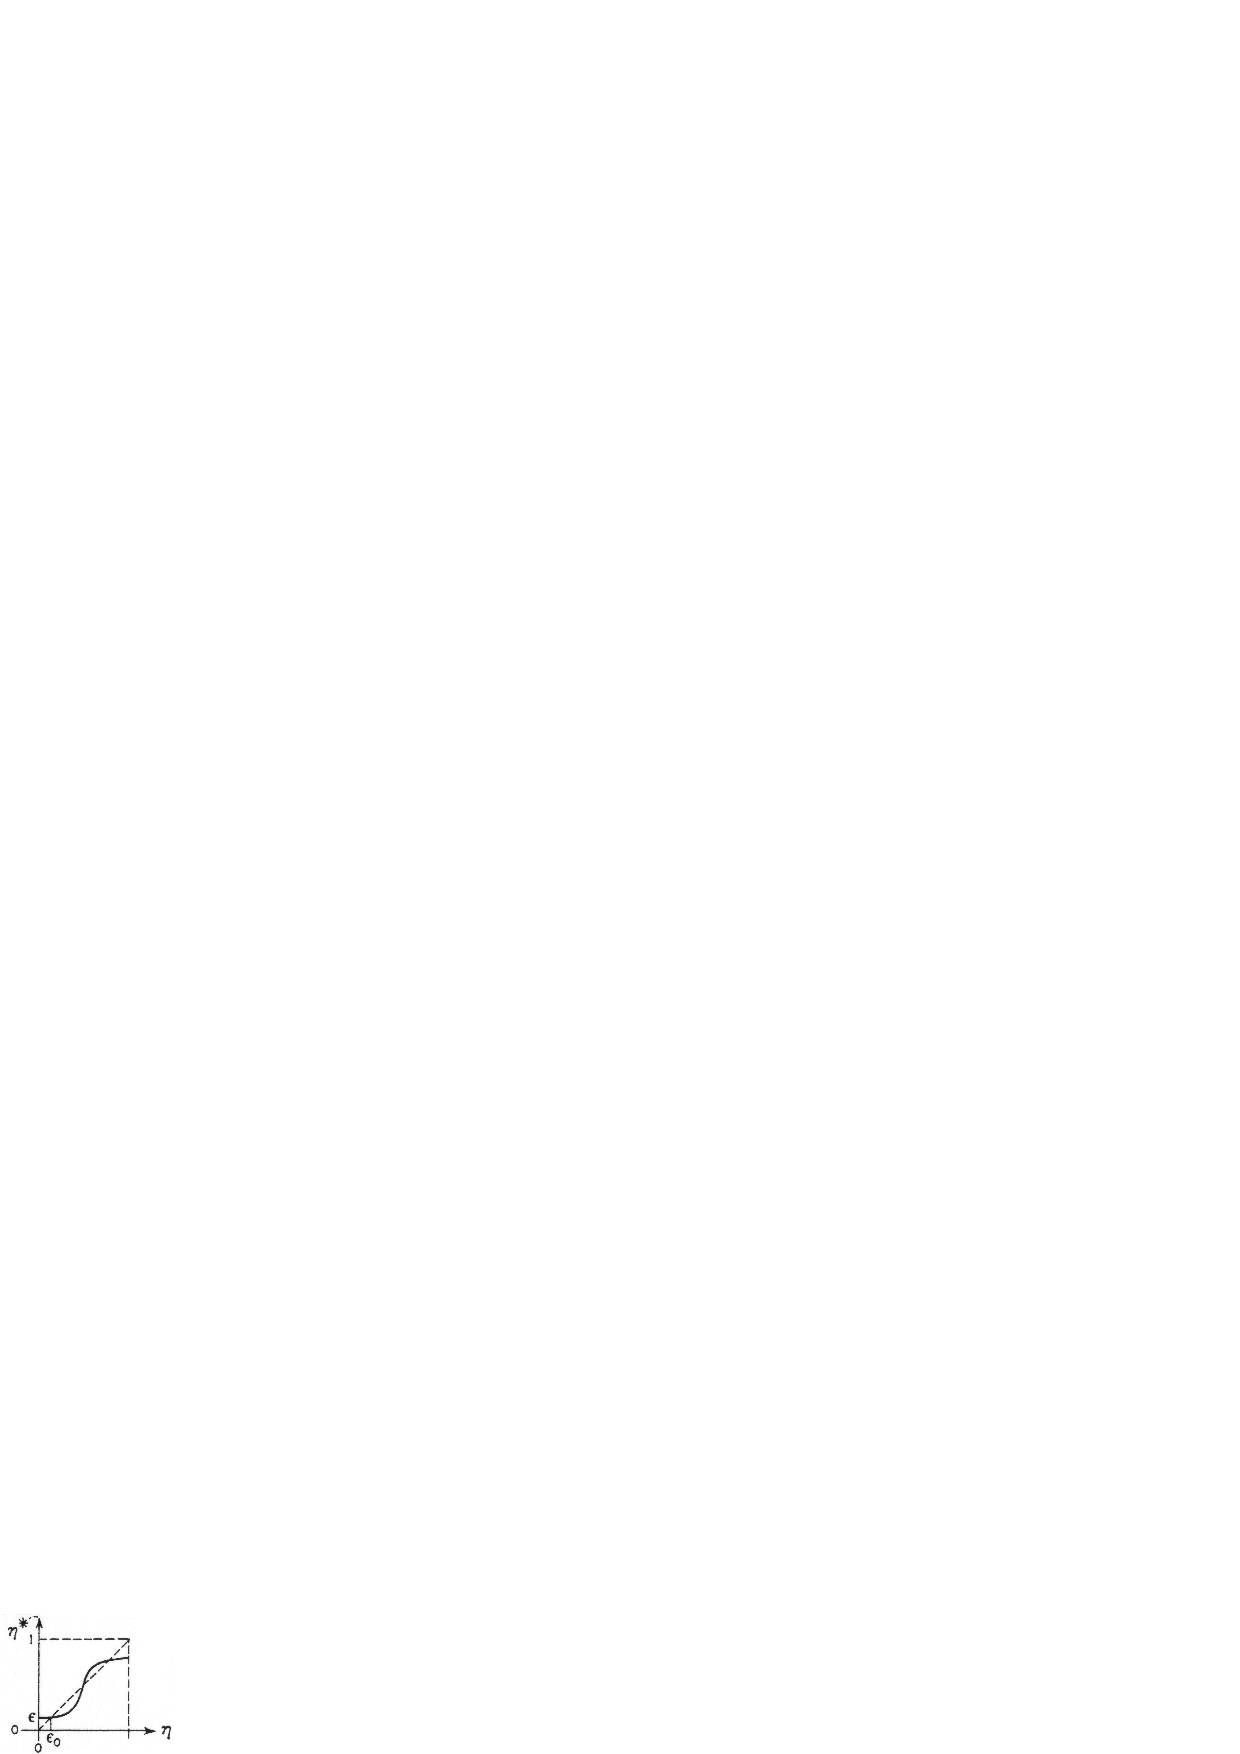
\includegraphics[width=2.4in]{fig_27}
\caption{\label{fig:27}}
\end{figure}

\subsubsection{\label{sec:eight3_2}The Rigorous Argument}

\begin{figure*}

\includegraphics[width=5.6in]{fig_28}
\caption{\label{fig:28}}
\end{figure*}

To make this heuristic argument binding, it would be necessary to
construct an error controlling network $P^*$ for any given network
$P$, so that all basic organs in $P^*$ are so connected as to put
them into the special case for a majority organ, as discussed
above. This will not be uniformly possible, and will therefore be
necessary to modify the above heuristic argument, although its
general pattern will be maintained.

It is, then desired, to find for any given network $P$ an
essentially equivalent network $P^*$, which is error-safe in some
suitable sense, that conforms with the ideas expressed so far. We
will define this as meaning, that for each output line of $P^*$
(corresponding to one of $P$) the (separate) probability of an
incorrect message (over this line) is $\leq \eta_1$. The value of
$\eta_1$ will result from the subsequent discussion.

The construction will be an induction over the longest serial
chain of basic organs in $P$, say $\mu=\mu(P)$.

Consider the structure of $P$. The number of its inputs $i$ and
outputs $\sigma$ is arbitrary, but every output of $P$ must either
come from a basic organ in $P$, or directly from an input, or from
a ground or live source. Omit the first mentioned basic organs
from $P$, as well as the outputs other than the first mentioned
ones, and designate the network that is left over by $Q$. This is
schematically shown in Figure~\ref{fig:28}. (Some of the
apparently separate outputs of $Q$ may be split lines coming from
a single one, but this is irrelevant for what follows.)

If $Q$ is void, then there is nothing to prove; let therefore $Q$
be non-void. Then clearly $\mu(Q)=\mu(P)-1$.

Hence the induction permits us to assume the existence of a
network $Q^*$ which is essentially equivalent to $Q$, and has for
each output a (separate) error-probability $\leq \eta_1$.

We now provide three copies of $Q^*$: $Q^{*1}$, $Q^{*2}$,
$Q^{*3}$, and construct $P^*$ as shown in Figure~\ref{fig:29}.
(Instead of drawing the, rather complicated, connections across
the two dotted areas, they are indicated by attaching identical
markings to endings that should be connected.)

Now the (separate) output error-probabilities of $Q^*$ are (by
inductive assumption) $\leq\eta_1$. The majority organs in the
first column in the above figure (those without a $\Box$) are so
connected as to belong into the special case for a majority organ
(cf. \ref{sec:eight2}), hence their outputs have (separate)
error-probabilities $\leq f_\epsilon(\eta_1)$. The majority organs
in the second column in the above figure (those with a $\Box$) are
in the general case, hence their (separate) error-probabilities
are $\leq\epsilon+3f_\epsilon(\eta_1)$.

\begin{figure*}
\includegraphics[width=5.4in]{fig_29}
\caption{\label{fig:29}}
\end{figure*}

Consequently the inductive step succeeds, and therefore the
attempted inductive proof is binding, if

\begin{equation}
\epsilon+3\epsilon f_\epsilon(\eta_1)\leq\eta_1~.\label{eq:12}
\end{equation}

\subsection{\label{sec:eight4}Numerical Evaluation}

Substituting the expression Eq.~\ref{eq:9} for $f_\epsilon(\eta)$
into condition Eq.~\ref{eq:9} gives

\begin{equation*}
4\epsilon+3(1-2\epsilon)(3\eta_1^2-2\eta_1^3)\leq\eta_1~,
\end{equation*}

\noindent i.e.,

\begin{equation*}
\eta_1^3-\frac{3}{2}\eta_1^2+\frac{1}{6(1-2\epsilon)}\eta_1-\frac{2\epsilon}{3(1-2\epsilon)}\geq0~.
\end{equation*}

\noindent Clearly the smallest $\eta_1>0$ fulfilling this
condition is wanted. Since the left hand side is $<0$ for
$\eta_1\leq0$, this means the smallest (real, and hence, by the
above, positive) root of

\begin{equation}
\eta_1^3-\frac{3}{2}\eta_1^2+\frac{1}{6(1-2\epsilon)}\eta_1-\frac{2\epsilon}{3(1-2\epsilon)}=0~.
\label{eq:13}
\end{equation}

\noindent We know from the preceding heuristic argument, that
$\epsilon\leq1/6$ will be necessary - but actually even more must
be required. Indeed, for $\eta_1=1/2$ the left hand side of
Eq.~\ref{eq:13} is $=-(1+\epsilon)/(6-12\epsilon)<0$, hence a
significant and acceptable $\eta_1$ (i.e., an $\eta_1<1/2$), can
be obtained from Eq.~\ref{eq:13} only if it has three real roots.
A simple calculation shows, that for $\epsilon=1/6$ only one real
root exists $\eta_1=1.425$. Hence the limiting $\epsilon$ calls
for the existence of a double root. Further calculation shows,
that the double root in question occurs for $\epsilon=0.0073$, and
that its value is $\eta_1=0.060$. Consequently $\epsilon < 0.0073$
is the actual requirement, i.e., the error-level of a single basic
organ function must be $< 0.73\%$. The stable, ultimate
error-level is then the smallest positive root $\eta_1$ of
Eq.~\ref{eq:13}. $\eta_1$ is small if $\epsilon$ is, hence
$\epsilon$ must be small, and so (from Eq.~\ref{eq:13})

\begin{equation*}
\eta_1=4\epsilon+152\epsilon^2+\dots~.
\end{equation*}

\noindent It is easily seen, that e.g. an ultimate error-level of
$2\%$ (i.e., $\eta_1=0.02$) calls for a single basic organ
function error-level of $0.41\%$ (i.e., $\epsilon=0.0041$).

This result shows that errors can be controlled. But the method of
construction used in the proof about threefolds the number of
basic organs in $P^*$ for an increase of $\mu(P)$ by 1, hence
$P^*$ has to contain about $3^{\mu(P)}$ such organs. Consequently
the procedure is impractical.

The restriction $\epsilon<0.0073$ has no absolute significance. It
could be relaxed by iterating the process of triplication at each
step. The inequality $\epsilon < 1/6$ is essential, however, since
our first argument showed, that for $\epsilon\geq1/6$ even for a
basic organ in the most favorable situation (namely in the
``special" one) no interval of improvement exists.

\section{\label{sec:nine}The Technique of Multiplexing}

\subsection{\label{sec:nine1}General Remarks on Multiplexing}

The general process of multiplexing in order to control error was
already referred to in \ref{sec:seven4}. The messages are carried
on $N$ lines. A positive number $\Delta$ ($<1/2$) is chosen and
the stimulation of $\geq (1-\Delta)N$ lines of the bundle is
interpreted as a positive message, the stimulation of $\leq \Delta
N$ lines as a negative message. Any other number of stimulated
lines is interpreted as a malfunction. The complete system must be
organized in such a manner, that a malfunction of the whole
automaton cannot be caused by the malfunctioning of a single
component, or of a small number of components, but only by the
malfunctioning of a large number of them. As we will see later,
the probability of such occurrences can be made arbitrarily small
provided the number of lies in each bundle is made sufficiently
great. All of section~\ref{sec:nine} will be devoted to a
description of the method of constructing multiplexed automata and
its discussion, without considering the possibility of error in
the basic components. In section~\ref{sec:ten} we will then
introduce errors in the basic components, and estimate their
effects.

\subsection{\label{sec:nine2}The Majority Organ}

\subsubsection{\label{sec:nine2_1}The Basic Executive Organ} The
first thing to consider is the method of constructing networks
which will perform the tasks of the basic organs for bundles of
inputs and outputs instead of single lines.

A simple example will make the process clear. Consider the problem
of constructing the analog of the majority organ which will
accommodate bundles of five lines. This is easily done using the
ordinary majority organ of Figure~\ref{fig:12}, as shown in
Figure~\ref{fig:30}. (The connections are replaced by suitable
markings, in the same way as in Figure~\ref{fig:29}.)

\begin{figure}
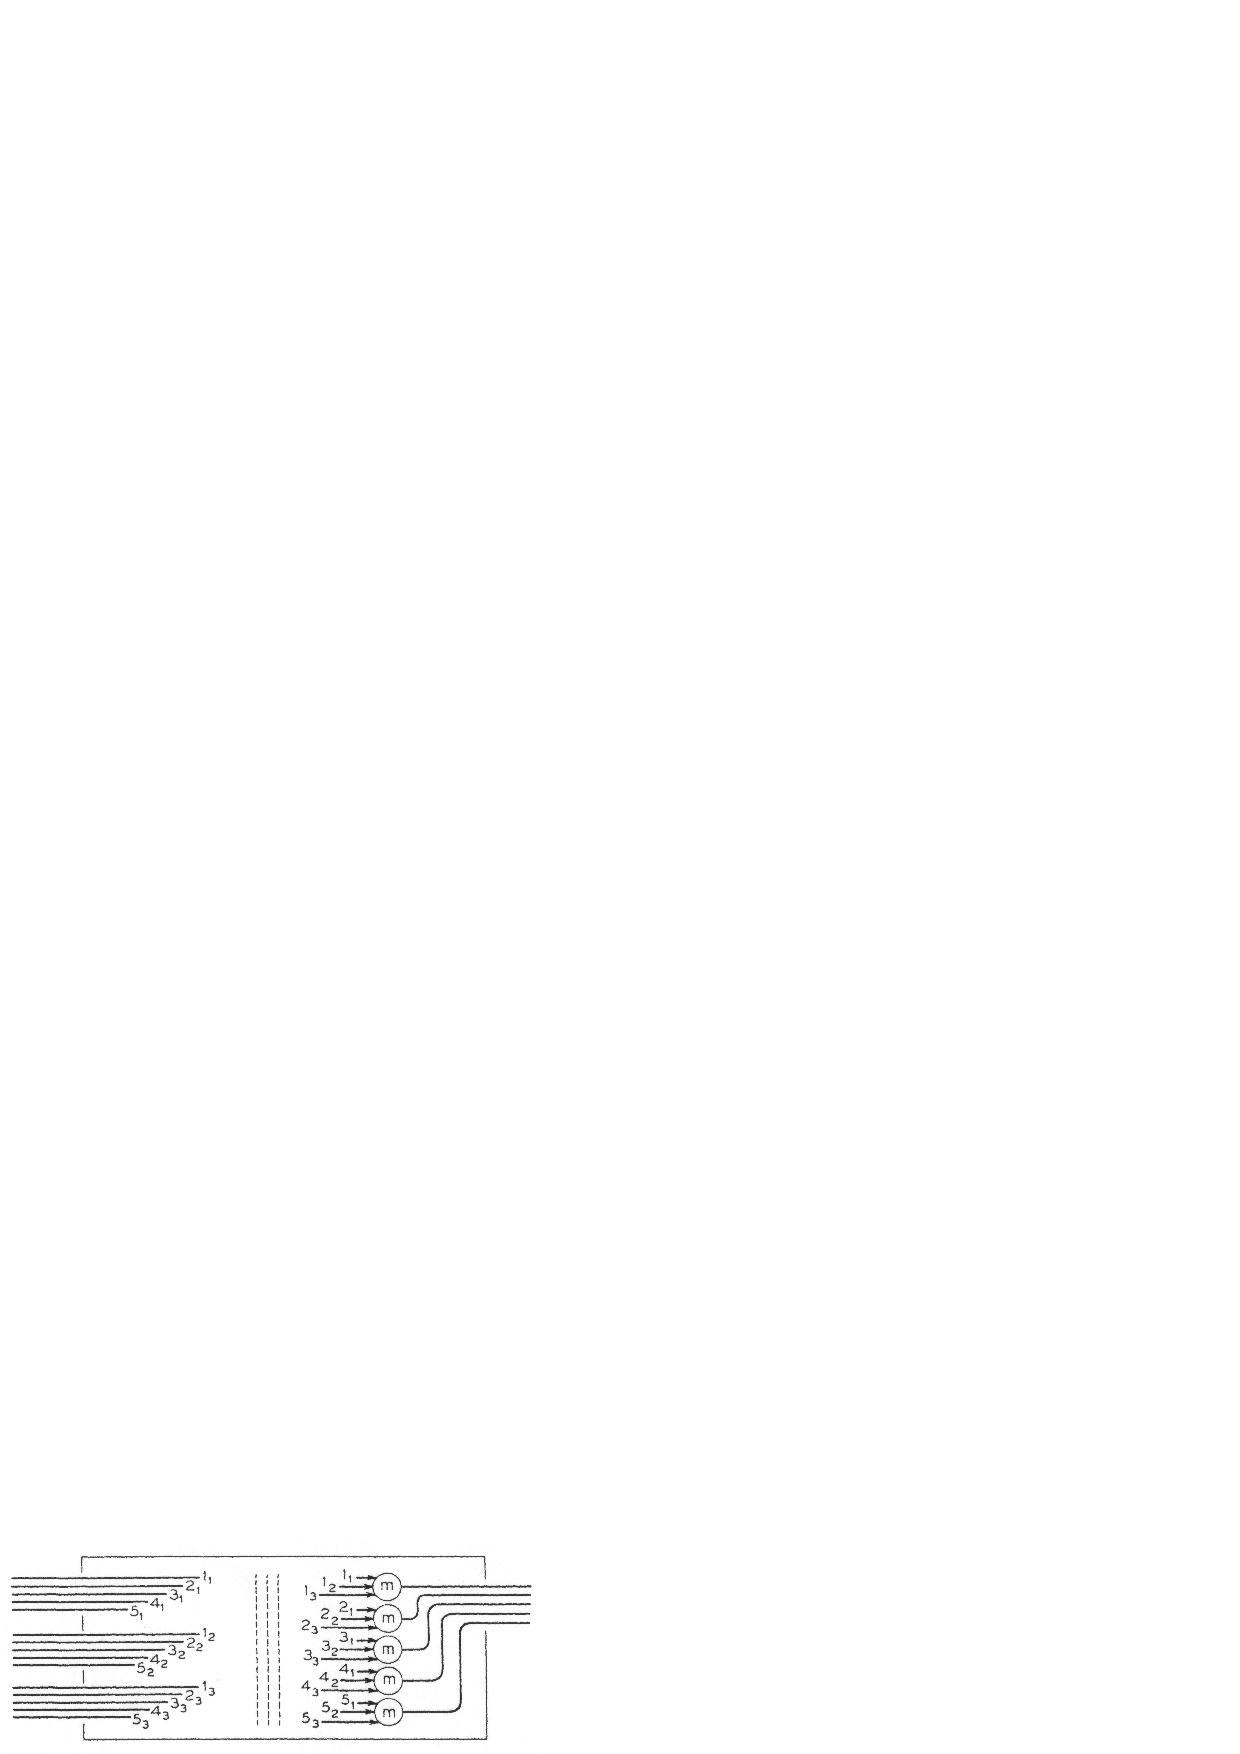
\includegraphics[width=3.4in]{fig_30}
\caption{\label{fig:30}}
\end{figure}

\subsubsection{\label{sec:nine2_2}The Need for a Restoring Organ}
It is intuitively clear that if almost all lines of two of the
inputs bundles are stimulated, then almost all lines of the output
bundle will be stimulated. Similarly if almost none of the lines
of two of the input bundles are stimulated, then the mechanism
will stimulate almost none of its output lines. However, another
fact is brought to light. Suppose that a critical level
$\Delta=1/5$ is set for the bundles. Then if two of the input
bundles have 4 lines stimulated while the other has none, the
output may have only 3 lines stimulated. The same effect prevails
in the negative case. If two bundles have just one inputs each
stimulated, while the third bundle has all of its inputs
stimulated, then the resulting output may be the stimulation of
two lines. In other words, the relative number of lines in the
bundle, which are not in the majority state, can double in passing
through the generalized majority system. A more careful analysis
(similar to the one that will be gone into in more detail for the
case of the Sheffer organ in \ref{sec:ten}) shows the following:
If, in some situation, the operation of the organ should be
governed by a two-to-one majority of the input bundles (i.e., if
two of these bundles are both prevalently stimulated or both
prevalently non-stimulated, while the third one is in the opposite
condition), then the most probable level of the output error will
be (approximately) the sum of the errors in the two governing
input bundles; on the other hand, in an operation in which the
organ is governed by a unanimous behavior of its input bundles
(i.e., if all three of these bundles are prevalently stimulated or
all three are prevalently non-stimulated), then the output error
will generally be smaller than the (maximum of the) input errors.
Thus in the significant case of two-to-one majorization, two
significant inputs may combine to produce a result lying in the
intermediate region of uncertain information. What is needed
therefore, is a new type of organ which will restore the original
stimulation level which is near to zero or to one into an output
bundle with stimulation level which is even closer to the
corresponding extreme.

Thus the multiplexed systems must contain two types of organs. The
first type is the executive organ which performs the desired basic
operations on the bundles. The second type is an organ which
restores the stimulation level of the bundles, and hence erases
the degradation caused by the executive organs. This situation has
its analog in many of the real automata which perform logically
complicated tasks. For example in electrical circuits, some of the
vacuum tubes perform executive functions, such as detection or
rectification of gating or coincidence-sensing, while the remainer
are assigned the task of amplification, which is a restorative
operation.

\subsubsection{\label{sec:nine2_3}The Restoring Organ}

\noindent (i) \textsc{Construction}: The construction of a
restoring organ is quite simple in principle, and in fact
contained in the second remark made in \ref{sec:nine2_2}. In a
crude way, the ordinary majority organ already performs this task.
Indeed in the simplest case, for a bundle of three lines, the
majority organ has precisely the right characteristics: It
suppresses a single incoming impulse as well as a single incoming
non-impulse, i.e., it amplifies the prevalence of the presence as
well as the absence of impulses. To display this trait most
clearly, it suffices to split its output line into three lines, as
shown in Figure~\ref{fig:31}.

\begin{figure}[b]

\includegraphics[width=2.2in]{fig_31}
\caption{\label{fig:31}}
\end{figure}

Now for large bundles, in the sense of the remark referred to
above, concerning the reduction of errors in the case of a
response induced by a unanimous behavior of the input bundles, it
is possible to connect up majority organs in parallel and thereby
produce the desired restoration. However, it is necessary to
assume that the stimulated (or non-stimulated) lines are
distributed at random in the bundle. This randomness must then be
maintained at all times. The principle is illustrated by
Figure~\ref{fig:32}. The ``black box" \textsf{U} is supposed to
permute the lines of the input bundle that pass through it, so as
to restore the randomness of the pulses in its lines. This is
necessary, since to the left of \textsf{U} the input bundle
consists of a set of triads, where the lines of each triad
originate in the splitting of a single line, and hence are always
all three in the same condition. Yet, to the right of \textsf{U}
the lines of the corresponding triad must be statistically
independent, in order to permit the application of the statistical
formula to be given below for the functioning of the majority
organ into which they feed. The way to select such a randomizing
permutation will not be considered here - it is intuitively
plausible that most ``complicated" permutations will be suited for
this ``randomizing" role. (Cf. \ref{sec:eleven2}.)\\

\begin{figure}

\includegraphics[width=3.2in]{fig_32}
\caption{\label{fig:32}}
\end{figure}

\noindent (ii) \textsc{Numerical Evaluation}: If $\alpha N$ of the
$N$ incoming lines are stimulated, then the probability of any
majority organ being stimulated (by two or three stimulated
inputs) is

\begin{equation}
\alpha^*=3\alpha^2-2\alpha^3=g(\alpha)~. \label{eq:14}
\end{equation}

\noindent Thus approximately (i.e., with high probability,
provided $N$ is large) $\alpha^* N$ outputs will be excited.
Plotting the curve of $\alpha^*$ against $\alpha$, as shown in
Figure~\ref{fig:33}, indicates clearly that this organ will have
the desired characteristics:

\begin{figure}[b]
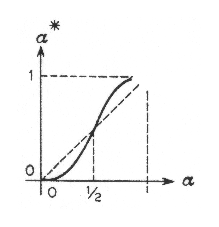
\includegraphics[width=2.4in]{fig_33}
\caption{\label{fig:33}}
\end{figure}

This curve intersects the diagonal $\alpha^*=\alpha$ three times:
For $\alpha=0$, $1/2$, $1$. $0<\alpha<1/2$ implies
$0<\alpha^*<\alpha$; $1/2<\alpha<1$ implies $\alpha<\alpha^*<1$.
I.e., successive iterates of this process converge to $0$ if the
original $\alpha<1/2$ and to $1$ if the original $\alpha>1/2$.

In other words: The error levels $\alpha\sim0$ and $\alpha\sim1$
will not only maintain themselves in the long run, but they
represent the asymptotic behavior for any original $\alpha<1/2$ or
$\alpha>1/2$, respectively. Note, that because of
$g(1-\alpha)\equiv1-g(\alpha)$ there is complete symmetry between
the $\alpha<1/2$ region and the $\alpha>1/2$ region.

The process $\alpha\rightarrow\alpha^*$ thus brings every $\alpha$
nearer to that one of 0 and 1, to which it was nearer originally.
this is precisely that process of restoration, which was seen in
\ref{sec:nine2_2} to be necessary. I.e., one or more (successive)
applications of this process will have the required restoring
effect.

Note, that this process of restoration is most effective when
$\alpha-\alpha^*=2\alpha^3-3\alpha^2+\alpha$ has its minimum or
maximum, i.e., for $6\alpha^2-6\alpha+1=0$, i.e., for
$\alpha=(3\pm\sqrt{3})/6=0.788$, $0.212$. Then
$\alpha-\alpha^*=\mp 0.096$. I.e., the maximum restoration is
effected on error levels at the distance of $21.2\%$ from $0\%$ or
$100\%$ - these are improved (brought nearer) by $9.6\%$.

\subsection{\label{sec:nine3}Other Basic Organs}

We have so far assumed that the basic components of the
construction are majority organs. From these, an analog of the
majority organ - one which picked out a majority of bundles
instead of a majority of single lines - was constructed. Since
this, when viewed as a basic organ, is a universal organ, these
considerations show that it is at least theoretically possible to
construct any network with bundles instead of single lines.
However there was no necessity for starting from majority organs.
Indeed, any other basic system whose universality was established
in section~\ref{sec:four} can be used instead. The simplest
procedure in such a case is to construct an (essential) equivalent
of the (single line) majority organ from the given basic system
(cf. \ref{sec:four2_2}), and then proceed with this composite
majority organ in the same way, as was done above with the basic
majority organ.

Thus, if the basic organs are those Nos. one and two in
Figure~\ref{fig:10} (cf. the relevant discussion in
\ref{sec:four1_2}), then the basic synthesis (that of the majority
organ, cf. above) is immediately derivable from the introductory
formula of Figure~\ref{fig:14}.

\subsection{\label{sec:nine4}The Sheffer Stroke}

\subsubsection{\label{sec:nine4_1}The Executive Organ} Similarly,
it is possible to construct the entire mechanism starting from the
Sheffer organ of Figure~\ref{fig:12}. In this case, however, it is
simpler not to effect the passage to an (essential) equivalent of
the majority organ (as suggested above), but to start \textit{de
novo}. Actually, the same procedure, which was seen above to work
for the majority organ, works \textit{mutatis mutandis} for the
Sheffer organ, too. A brief description of the direct procedure in
this case is given in what follows:

Again, one begins by constructing a network which will perform the
task of the Sheffer organ for bundles of inputs and outputs
instead of single lines. This is shown in Figure~\ref{fig:34} for
bundles of five wires. (The connections are replaced by suitable
markings, as in Figures~\ref{fig:29} and \ref{fig:30}.)

\begin{figure}
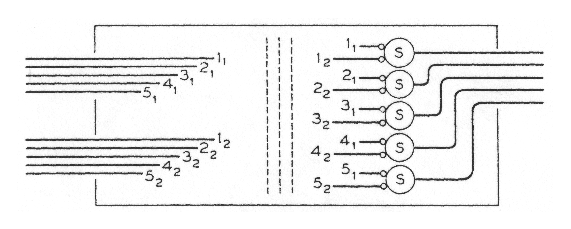
\includegraphics[width=3.3in]{fig_34}
\caption{\label{fig:34}}
\end{figure}

It is intuitively clear that if almost all lines of both input
bundles are stimulated, then almost none of the lines of the
output bundle will be stimulated. Similarly, if almost none of the
lines of one input bundle are stimulated, then almost all lines of
the output bundle will be stimulated. Similarly, if almost none of
the lines of one input bundle are stimulated, then almost all
lines of the output bundle will be stimulated. In addition to this
overall behavior, the following detailed behavior is found (cf.
the detailed consideration in \ref{sec:ten4}). If the condition of
the organ is one of prevalent non-stimulation of the output
bundle, and hence is governed by (prevalent stimulation of) both
input bundles, then the most probable level of the output error
will be (approximately) the sum of the errors in the two governing
input bundles; if on the other hand the condition of the organ is
one of prevalent stimulation of the output bundle, and hence is
governed by (prevalent non-stimulation of ) one or of both input
bundles, then the output error will be on (approximately) the same
level as the input error, if (only) one input bundle is governing
(i.e., prevalently non-stimulated), and it will be generally
smaller than the input error, if both input bundles are governing
(i.e., prevalently non-stimulated). Thus two significant inputs
may produce a result lying in the intermediate zone of uncertain
information. Hence a restoring organ (for the error level) is
again needed, in addition to the executive organ.

\subsubsection{\label{sec:nine4_2}The Restoring Organ} Again, the
above indicates that the restoring organ can be obtained from a
special case functioning of the standard executive organ, namely
by obtaining all inputs from a single input bundle, and seeing to
it that the output bundle has the same size as the original input
bundle. The principle is illustrated by Figure~\ref{fig:35}. The
``black box" \textsf{U} is again supposed to effect a suitable
permutation of the lines that pass through it, for the same
reasons and in the same manner as in the corresponding situation
for the majority organ (cf. Figure~\ref{fig:32}). I.e., it must
have a ``randomizing" effect.

\begin{figure}[b]
\includegraphics[width=3.2in]{fig_35}
\caption{\label{fig:35}}
\end{figure}

If $\alpha N$ of the $N$ incoming lines are stimulated, then the
probability of any Sheffer organ being stimulated (by at least one
non-stimulated input) is

\begin{equation}
\alpha^+=1-\alpha^2\equiv h(\alpha)~. \label{eq:15}
\end{equation}

\noindent Thus approximately (i.e., with high probability provided
$N$ is large) $\sim \alpha^+N$ outputs will be excited. Plotting
the curve of $\alpha^+$ against $\alpha$ discloses some
characteristic differences against the previous case (that one of
the majority organs, i.e., $\alpha^*=3\alpha^2-2\alpha^3\equiv
g(\alpha)$, cf. \ref{sec:nine2_3}), which require further
discussion. This curve is shown in Figure~\ref{fig:36}. Clearly
$\alpha^+$ is an antimonotone function of $\alpha$, i.e., instead
of restoring an excitation level (i.e., bringing it closer to 0 or
1, respectively), it transforms it into its opposite (i.e., it
brings the neighborhood of 0 close to 1, and the neighborhood of 1
close to 0). In addition it produces for $\alpha$ near to 1 an
$\alpha^+$ much nearer to 1 (second order!). All these
circumstances suggest, that the operation should be iterated.

\begin{figure}
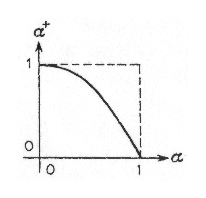
\includegraphics[width=2.1in]{fig_36}
\caption{\label{fig:36}}
\end{figure}

Let the restoring organ therefore consist of two of the previously
pictured organs in series, as shown in Figure~\ref{fig:37}. (The
``black boxes" $\textsf{U}_1$, $\textsf{U}_2$ play the same role
as their analog \textsf{U} plays in Figure~\ref{fig:35}.) This
organ transforms an inputs excitation level $\alpha N$ into an
output excitation level of approximately (cf. above) $\sim
\alpha^{++}$ where

\begin{equation*}
\alpha^{++}=1-(1-\alpha^2)^2\equiv h(h(\alpha))\equiv k(\alpha)~,
\end{equation*}

\noindent i.e.,

\begin{equation}
\alpha^{++}=2\alpha^2-\alpha^4\equiv k(\alpha)~. \label{eq:16}
\end{equation}

\noindent This curve of $\alpha^{++}$ against $\alpha$ is shown in
Figure~\ref{fig:38}. This curve is very similar to that one
obtained for the majority organ (i.e.,
$\alpha^*=3\alpha^2-2\alpha^3\equiv g(\alpha)$, cf.
\ref{sec:nine2_3}). Indeed: The curve intersects the diagonal
$\alpha^{++}=\alpha$ in the internal $0\leq \alpha \leq 1$ three
times: For $\alpha=0$, $\alpha_0$, 1, where
$\alpha_0=(-1+\sqrt{5})/2=0.618$. (There is a fourth intersection
$\alpha=-1-\alpha_0=-1.618$, but this is irrelevant, since it is
not in the interval $0\leq\alpha\leq1$.) $0<\alpha<\alpha_0$
implies $0<\alpha^{++}<\alpha$; $\alpha_0<\alpha<1$ implies
$\alpha<\alpha^{++}<1$.

\begin{figure*}
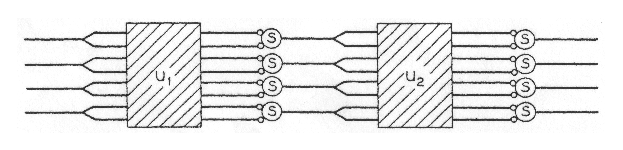
\includegraphics[width=5.4in]{fig_37}
\caption{\label{fig:37}}
\end{figure*}

\begin{figure}[b]
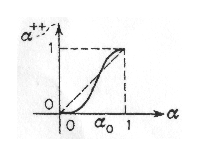
\includegraphics[width=2.6in]{fig_38}
\caption{\label{fig:38}}
\end{figure}

In other words: The role of the error levels $\alpha\sim0$ and
$\alpha\sim1$ is precisely the same as for the majority organ (cf.
\ref{sec:nine2_3}), except that the limit between their respective
areas of control lies at $\alpha=\alpha_0$ instead of at
$\alpha=1/2$. I.e., the process $\alpha\rightarrow\alpha^{++}$
brings every $\alpha$ nearer to either 0 or to 1, but the
preference to 0 or 1 is settled at a discrimination level of
$61.8\%$ (i.e., $\alpha_0$) instead of one of $50\%$ (i.e.,
$1/2$). Thus, apart from a certain asymmetric distortion, the
organ behaves like its counterpart considered for the majority
organ - i.e., it is an effective restoring mechanism.

\section{\label{sec:ten}Error in Multiplex Systems}

\subsection{\label{sec:ten1}General Remarks}

In section~\ref{sec:nine} the technique for constructing
multiplexed automata was described. However, the role of errors
entered at best intuitively and summarily, and therefore it has
still not been proved that these systems will do what is claimed
for them - namely control error. Section~\ref{sec:ten} is devoted
to a sketch of the statistical analysis necessary to show that, by
using large enough bundles of lines, any desired degree of
accuracy (i.e., as small a probability of malfunction of the
ultimate output of the network as desired) can be obtained with a
multiplexed automaton.

For simplicity, we will only consider automata which are
constructed from the Sheffer organs. These are easier to analyze
since they involve only two inputs. At the same time, the Sheffer
organ is (by itself) universal (cf. \ref{sec:four2_1}), hence
every automaton is essentially equivalent to a network of Sheffer
organs.

Errors in the operation of an automaton arise from two sources.
First, the individual basic organs can make mistakes. It will be
assumed as before, that, under any circumstances, the probability
of this happening is just $\epsilon$. Any operation on the bundle
can be considered as a random sampling of size $N$ ($N$ being the
size of the bundle). The number of errors committed by the
individual basic organs in any operation on the bundle is then a
random variable, distributed approximately normally with mean
$\epsilon N$ and standard deviation
$\sqrt{\epsilon(1-\epsilon)N}$. A second source of failures arises
because in operating with bundles which are not all in the same
state of stimulation or non-stimulation, the possibility of
multiplying error by unfortunate combinations of lines into the
basic (single line) organs is always present. This intersects with
the statistical effects, and in particular with the processes of
degeneration and of restoration of which we spoke in
\ref{sec:nine2_2}, \ref{sec:nine2_3} and \ref{sec:nine4_2}.

\subsection{\label{sec:ten2}The Distribution of the Response Set Size}

\subsubsection{\label{sec:ten2_1}Exact Theory} In order to give a
statistical treatment of the problem, consider the
Figure~\ref{fig:34}, showing a network of Sheffer organs, which
was discussed in \ref{sec:nine4_1}. Let again $N$ be the number of
lines in each (input or output) bundle. Let $X$ be the set of
those $i=1,\dots,N$ for which line No. $i$ in the first input
bundle is stimulated at time $t$; let $Y$ be the corresponding set
for the second input bundle and time $t$; and let $Z$ be the
corresponding set for the output bundle, assuming the correct
functioning of all the Sheffer organs involved, and time $t+1$.
Let $X$, $Y$ have $\xi N$, $\eta N$ elements, respectively, but
otherwise be random - i.e., equidistributed over all pairs of sets
with these numbers of elements. What can then be said about the
number of elements $\zeta N$ of $Z$? Clearly $\xi$, $\eta$,
$\zeta$, are the relative levels of excitation of the two input
bundles and of the output bundle, respectively, of the network
under consideration. The question is then: What is the
distribution of the (stochastic) variable $\zeta$ in terms of the
(given) $\xi$, $\eta$?

Let $W$ be the complementary set of $Z$. Let $p$, $q$, $r$ be the
numbers of elements of $X$, $Y$, $W$, respectively, so that $p=\xi
N$, $q=\eta N$, $r=(1-\zeta)N$. Then the problem is to determine
the distribution of the (stochastic) variable $r$ in terms of the
(given) $p$, $q$ - i.e., the probability of any given $r$ in
combination with any given $p$, $q$.

$W$ is clearly the intersection of the sets $X$, $Y$: $W=X\cdot
Y$. Let $U$, $V$ be the (relative) complements of $W$ in $X$, $Y$,
respectively: $U=X-W$, $V=Y-W$, and let $S$ be the (absolute,
i.e., in the set (1,\dots,N)) complement of the sum of $X$ and
$Y$: $S=N+W-(X+W)$. Then $W$, $U$, $V$, $S$ are pairwise disjoint
sets making up together precisely the entire set $(1,\ldots,N)$,
with $r$, $p-r$, $q-r$, $N-p-q+r$ elements, respectively. Apart
from this they are unrestricted. Thus they offer together
$N!/[r!(p-r)!(q-r)!(N-p-q+r)!]$ possible choices. Since there are
\textit{a priori} $N![p!(N-p)!]$ possible choices of an $X$ with
$p$ elements and \textit{a priori} $N!/[q!(N-q)!$ possible choices
of a $Y$ with $q$ elements, this means that the looked for
probability of $W$ having $r$ elements is

\begin{eqnarray*}
\rho & = & \left( \frac{N!}{r!(p-r)!(q-r)!(N-p-q+r)!} \right \\
     &   & \left \diagup\frac{N!}{p!(N-p)!} \frac{N!}{q!(N-q)!}
     \right)\\
     & = & \frac{p!(N-p)!q!(N-q)!}{r!(p-r)!(q-r)!(N-p-q+r)!N!}~.
\end{eqnarray*}

Note that this formula also shows that $\rho=0$ when $r<0$ or
$p-r<0$ or $q-r<0$ or $N-p-q+r<0$, i.e., when $r$ violates the
conditions

\begin{equation*}
\mathrm{Max}(0, p+q-N)\leq r \leq \mathrm{Min}(p, q)~.
\end{equation*}

\noindent This is clear combinatorially, in view of the meaning of
$X$, $Y$ and $W$. In terms of $\xi$, $\eta$, $\zeta$ the above
conditions become

\begin{equation}
\label{eq:17} 1-\mathrm{Max}(0, \xi+\eta-1)\geq \zeta \geq
1-\mathrm{Min}(\xi, \eta)~.
\end{equation}

Returning to the expression for $\rho$, substituting the $\xi$,
$\eta$, $\zeta$ expressions for $p$, $q$, $r$ and using Stirling's
formula for the factorials involved, gives

\begin{equation}
\label{eq:18} \rho\sim\frac{1}{\sqrt{2\pi
N}}\sqrt{a}\mathrm{e}^{-\theta N}~,
\end{equation}

\noindent where

\begin{eqnarray*}
a & = &
\frac{\xi(1-\xi)\eta(1-\eta)}{(\zeta+\xi-1)(\zeta+\eta-1)(1-\zeta)(2-\xi-\eta-\zeta)}\\\\
\theta & = & (\zeta+\xi-1)\ln{(\zeta+\xi-1)}+(\zeta+\eta-1)\ln{(\zeta+\eta-1)}\\
       &   & +
       (1-\zeta)\ln{(1-\zeta)}+(2-\xi-\eta-\zeta)\ln{(2-\xi-\eta-\zeta)}\\
       &   &
       -\xi\ln{\xi}-(1-\xi)\ln{(1-\xi)}-\eta\ln{\eta}-(1-\eta)\ln{(1-\eta)}~.
\end{eqnarray*}

\noindent From this

\begin{eqnarray*}
\begin{array}{c}
\frac{\partial\theta}{\partial\zeta}=\ln{\frac{(\zeta+\xi-1)(\zeta+\eta-1)}{(1-\zeta)(2-\xi-\eta-\zeta)}}~,\\\\
\frac{\partial^2\theta}{\partial\zeta^2}=\frac{1}{\zeta+\xi-1)}+\frac{1}{\zeta+\eta-1}+\frac{1}{1-\zeta}+\frac{1}{2-\xi-\eta-\zeta}~.
\end{array}
\end{eqnarray*}

Hence $\theta=0$, $\frac{\partial\theta}{\partial\zeta}=0$ for
$\zeta=1-\xi\eta$, and $\partial^2\theta/\partial\zeta^2>0$ for
all $\zeta$ (in its entire interval of variability according to
Eq.~\ref{eq:17}). This implies, in view of Eq.~\ref{eq:18} that
for all $\zeta$ which are significantly $\neq 1-\xi\eta$, $\rho$
tends to 0 very rapidly as $N$ gets large. It suffices therefore
to evaluate Eq.~\ref{eq:18} for $\zeta\sim1-\xi\eta$. Now
$a=1/[\xi(1-\xi)\eta(1-\eta)]$,
$\partial^2\theta/\partial\zeta^2=1/[\xi(1-\xi)\eta(1-\eta)]$ for
$\zeta=1-\xi\eta$. Hence

\begin{eqnarray*}
a & \sim & \frac{1}{\xi(1-\xi)\eta(1-\eta)}~,\\\\
\theta & \sim &
\frac{(\zeta-(1-\xi\eta))^2}{2\xi(1-\xi)\eta(1-\eta)}
\end{eqnarray*}

\noindent for $\zeta\sim1-\xi\eta$. Therefore

\begin{equation}
\label{eq:19} \rho \sim
\frac{1}{\sqrt{2\pi\xi(1-\xi)\eta(1-\eta)N}}~\mathrm{e}^{-\frac{(\zeta-(1-\xi\eta))^2}{2\xi(1-\xi)\eta(1-\eta)}N}
\end{equation}

\noindent is an acceptable approximation for $\rho$.

$r$ is an integer-valued variable, hence $\zeta=1-\frac{r}{N}$ is
a rational-valued variable, with the fixed denominator $N$. Since
$N$ is assumed to be very large, the range of $\zeta$ is very
dense. It is therefore permissible to replace it by a continuous
one, and to describe the distribution of $\zeta$ by a
probability-density $\sigma$. $\rho$ is the probability of a
single value of $\zeta$, and since the values of $\zeta$ are
equidistant, with a separation $\mathrm{d}\zeta=1/N$, the relation
between $\sigma$ and $\rho$ is best defined by
$\sigma\mathrm{d}\zeta=\rho$, i.e., $\sigma=\rho N$. Therefore
Eq.~\ref{eq:19} becomes

\begin{equation}
\label{eq:20} \rho \sim
\frac{1}{\sqrt{2\pi}\sqrt{\xi(1-\xi)\eta(1-\eta)/N}}~\mathrm{e}^{-\frac{1}{2}{\left(\frac{\zeta-(1-\xi\eta)}{\sqrt{2\xi(1-\xi)\eta(1-\eta)/N}}\right)}^2}
\end{equation}

\noindent This formula means obviously the following:

$\zeta$ is approximately normally distributed, with the mean
$1-\xi\eta$ and the dispersion $\sqrt{\xi(1-\xi)\eta(1-\eta)/N}$.
Note, that the rapid decrease of the normal distribution function
(i.e., the right hand side of Eq.~\ref{eq:20}) with $N$ (which is
exponential!) is valid as long as $\zeta$ is near to $1-\xi\eta$,
only the coefficient of $N$ (in the exponent, i.e.,
$-\frac{1}{2}\{[\zeta-(1-\xi\zeta)]/\sqrt{\xi(1-\xi)\eta(1-\eta)/N}\}^2$
is somewhat altered as $\zeta$ deviates from $1-\xi$. (This
follows from the discussion of $\theta$ given above.)

The simple statistical discussion of \ref{sec:nine4} amounted to
attributing to $\zeta$ the unique value $1-\xi\eta$. We see now
that this is approximately true:

\begin{eqnarray}
\left\{
\begin{array}{l}
\zeta=(1-\xi\eta)+\delta\sqrt{[\xi(1-\xi)\eta(1-\eta)]/N}~,\\\\
\delta~$is a stochastic variable, normally distributed,$\\
$with the mean 0 and the dispersion 1.$
\end{array}
\label{eq:21}
\end{eqnarray}

\subsubsection{\label{sec:ten2_2}Theory with Errors} We must now
pass from $r$, $\zeta$, which postulate faultless functioning of
all Sheffer organs in the network, to $r'$, $\zeta'$ which
correspond to the actual functioning of all these organs - i.e.,
to a probability $\epsilon$ of error on each functioning. Among
the $r$ organs each of which should correctly stimulate its
output, each error reduces $r'$ by one unit. The number of errors
here is approximately normally distributed, with the mean
$\epsilon r$ and the dispersion $\sqrt{\epsilon(1-\epsilon)r}$
(cf. the remark made in \ref{sec:ten1}). Among the $N-r$ organs,
each of which should correctly not stimulate its output, each
error increases $r'$ by one unit. The number of errors here is
again approximately normally distributed, with the mean
$\epsilon(N-r)$, and the dispersion
$\sqrt{\epsilon(1-\epsilon)(N-r)}$ (cf. as above). Thus $r'-r$ is
the difference of these two (independent) stochastic variables.
Hence it, too, is approximately normally distributed, with the
mean $-\epsilon r + \epsilon(N-r)=\epsilon(N-2r)$, and the
dispersion

\begin{equation*}
\sqrt{(\sqrt{\epsilon(1-\epsilon)r})^2+(\sqrt{\epsilon(1-\epsilon)(N-r)})}=\sqrt{\epsilon(1-\epsilon)N}~.
\end{equation*}

\noindent I.e., (approximately)

\begin{equation*}
r'=r+2\epsilon(\frac{N}{2}-r)+\delta'\sqrt{\epsilon(1-\epsilon)N}~,
\end{equation*}

\noindent where $\delta'$ is normally distributed, with the mean 0
and the dispersion 1. From this

\begin{equation*}
\zeta'=\zeta+2\epsilon(\frac{1}{2}-\zeta)-\delta'\sqrt{\epsilon(1-\epsilon)/N}~,
\end{equation*}

\noindent and then by Eq.~\ref{eq:21}

\begin{eqnarray*}
\zeta' & = & (1-\xi\eta)+2\epsilon(\xi\eta-\frac{1}{2})\\
       & + & (1-2\epsilon)\delta\sqrt{\xi(1-\xi)\eta(1-\eta)/N}-\delta'\sqrt{\epsilon(1-\epsilon)/N}~.
\end{eqnarray*}

\noindent Clearly
$(1-2\epsilon)\delta\sqrt{\xi(1-\xi)\eta(1-\eta)/N}\sim\delta'\sqrt{\epsilon(1-\epsilon)/N}$,
too, is normally distributed, with the mean 0 and the dispersion

\begin{eqnarray*}
\sqrt{[(1-2\epsilon)\sqrt{\xi(1-\xi)\eta(1-\eta)/N}]^2+[\sqrt{\epsilon(1-\epsilon)/N}]^2}\\
=\sqrt{[(1-2\epsilon)^2\xi(1-\xi)\eta(1-\eta)+\epsilon(1-\epsilon)]/N}~.
\end{eqnarray*}

\noindent Hence Eq.~\ref{eq:21} becomes at last (we write again
$\zeta$ in place of $\zeta'$):

\begin{eqnarray}
\left\{\begin{array}{l} \zeta =
(1-\xi\eta)+2\epsilon(\xi\eta-\frac{1}{2})\\
+ \delta^*\sqrt{[(1-2\epsilon)^2\xi(1-\xi)\eta(1-\eta)+\epsilon(1-\epsilon)]/N}~,\\\\
\delta^*~$is a stochastic variable, normally distributed,$\\
$with the mean 0 and the dispersion 1.$ \end{array} \label{eq:22}
\end{eqnarray}

\subsection{\label{sec:ten3}The Restoring Organ}

This discussion equally covers the situations that are dealt with
in Figures~\ref{fig:35} and \ref{fig:37}, showing networks of
Sheffer organs in \ref{sec:nine4_2}.

Consider first Figure~\ref{fig:35}. We have here a single input
bundle of $N$ lines, and an output bundle of $N$ lines. However,
the two-way split and the subsequent ``randomizing" permutation
produce an input bundle of $2N$ lines and (to the right of
\textsf{U}) the even lines of this bundle on one hand, and its odd
lines on the other hand, may be viewed as two input bundles of $N$
lines each. Beyond this point the network is the same as that one
of Figure~\ref{fig:34}, discussed in \ref{sec:nine4_1}. If the
original input bundle had $\xi N$ stimulated lines, then each one
of the two derived input bundles will also have $\xi N$ stimulated
lines. (To be sure of this, it is necessary to choose the
``randomizing" permutation \textsf{U} of Figure~\ref{fig:35} in
such a manner, that it permutes the even lines among each other,
and the odd lines among each other. This is compatible with its
``randomizing" the relationship of the family of all even lines to
the family of all odd lines. Hence it is reasonable to expect,
that this requirement does not conflict with the desired
``randomizing" character of the permutation.) Let the output
bundle have $\xi N$ stimulated lines. Then we are clearly dealing
with the same case as in Eq.~\ref{eq:22}, except that it is
specialized to $\xi=\eta$. Hence Eq.~\ref{eq:22} becomes:

\begin{eqnarray}
\left\{\begin{array}{l}\begin{array}{lll} \zeta & = & (1-\xi^2)+2\epsilon(\xi^2-\frac{1}{2})\\
& & + \delta^*\sqrt{[(1-2\epsilon)^2(\xi(1-\xi))^2+\epsilon(1-\epsilon)]/N}~,\\\\
\end{array}
\\
\delta^*~$is a stochastic variable, normally distributed,$\\
$with the mean 0 and the dispersion 1.$ \end{array} \label{eq:23}
\end{eqnarray}

Consider next Figure~\ref{fig:37}. Three bundles are relevant
here: The input bundle at the extreme left, the intermediate
bundle issuing directly from the first tier of Sheffer organs, and
the output bundle, issuing directly from the second tier of
Sheffer organs, i.e., at the extreme right. Each one of these
three bundles consists of $N$ lines. Let the number of stimulated
lines in each bundle be $\zeta N$, $\omega N$, $\psi N$,
respectively. Then Eq.~\ref{eq:23} above applies, with its $\xi$,
$\zeta$ replaced first by $\zeta$, $\omega$, and second by
$\omega$, $\psi$:

\begin{eqnarray}
\left\{\begin{array}{l}\begin{array}{lll} \omega & = &
(1-\zeta^2)+2\epsilon(\zeta^2-\frac{1}{2})\\
& & + \delta^{**}\sqrt{[(1-2\epsilon)^2(\zeta(1-\zeta))^2+\epsilon(1-\epsilon)]/N}~,\\\\
\psi & = &
(1-\omega^2)+2\epsilon(\omega^2-\frac{1}{2})\\
& & + \delta^{***}\sqrt{[(1-2\epsilon)^2(\omega(1-\omega))^2+\epsilon(1-\epsilon)]/N}~,\\\\
\end{array}
\\
\delta^{**}, \delta^{***},~$are stochastic variables, independently$\\
$and normally distributed, with the mean 0 and$\\
$the dispersion 1.$ \end{array} \label{eq:24}
\end{eqnarray}

\subsection{\label{sec:ten4}Qualitative Evaluation of the Results}

In what follows, Eqs.~\ref{eq:22} and \ref{eq:24} will be relevant
- i.e., the Sheffer organ networks of Figures~\ref{fig:34} and
\ref{fig:37}.

Before going into these considerations, however, we have to make
an observation concerning Eq.~\ref{eq:22}. Eq.~\ref{eq:22} shows
that the (relative) excitation levels $\xi$, $\eta$ on the input
bundles of its network generate approximately (i.e., for large $N$
and small $\epsilon$) the (relative) excitation level
$\zeta_0=1-\xi\eta$ on the output bundle of that network. This
justifies the statements made in \ref{sec:nine4_1} about the
detailed functioning of the network. Indeed: If the two input
bundles are both prevalently stimulated, i.e., if $\xi\sim1$,
$\eta\sim1$ then the distance of $\zeta_0$ from 0 is about the sum
of the distances of $\xi$ and of $\eta$ from 1:
$\zeta_0=(1-\xi)+\xi(1-\eta)$. If one of the two input bundles,
say the first one, is prevalently non-stimulated, while the other
one is prevalently stimulated., i.e., if $\xi\sim0$, $\eta\sim1$,
then the distance of $\zeta_0$ from 1 is about the distance of
$\xi$ from 0: $1-\zeta_0=\xi\eta$. If both input bundles are
prevalently non-stimulated, i.e., if $\xi\sim0$, $\eta\sim0$, then
the distance of $\zeta_0$ from 1 is small compared to the
distances of both $\xi$ and $\eta$ from 0: $1-\zeta_0-\xi\eta$.

\subsection{\label{sec:ten5}Complete Quantitative Theory}

\subsubsection{\label{sec:ten5_1}General Results} We can now pass
to the complete statistical analysis of the Sheffer stroke
operation on bundles. In order to do this, we must agree on a
systematic way to handle this operation by a network. The system
to be adopted will be the following: The necessary executive organ
will be followed in series by a restoring organ. I.e., the Sheffer
organ network of Figure~\ref{fig:34} will be followed in series by
the Sheffer organ network of Figure~\ref{fig:37}. This means that
the formulas of Eq.~\ref{eq:22} are to be followed by those of
Eq.~\ref{eq:24}. Thus $\xi$, $\eta$ are the excitation levels of
the two input bundles, $\psi$ is the excitation level of the
output bundle, and we have:

\begin{widetext}
\begin{eqnarray} \label{eq:25}\left\{\begin{array}{l}
\begin{array}{lll}\zeta & = & (1-\xi\eta)+2\epsilon(\xi\eta-\frac{1}{2}) + \delta^*\sqrt{[(1-2\epsilon)^2\xi(1-\xi)\eta(1-\eta)+\epsilon(1-\epsilon)]/N}~,\\\\
\omega & = & (1-\zeta^2)+2\epsilon(\zeta^2-\frac{1}{2}) + \delta^{**}\sqrt{[(1-2\epsilon)^2(\zeta(1-\zeta))^2+\epsilon(1-\epsilon)]/N}~,\\\\
\psi & = & (1-\omega^2)+2\epsilon(\omega^2-\frac{1}{2}) + \delta^{***}\sqrt{[(1-2\epsilon)^2(\omega(1-\omega))^2+\epsilon(1-\epsilon)]/N}~,\\\\
\end{array}
\\
\delta^*, \delta^{**}, \delta^{***},~$are stochastic variables, independently and normally $\\
$distributed, with the mean 0 and the dispersion 1.$\\
\end{array}
\end{eqnarray}
\end{widetext}

Consider now a given fiduciary level $\Delta$. Then we need a
behavior like the ``correct" one of the Sheffer stroke, with an
overwhelming probability. This means: The implication of
$\psi\leq\Delta$ by $\xi\geq1-\Delta$, $\eta\geq1-\Delta$; the
implication of $\psi\geq1-\Delta$ by $\xi\leq\Delta$,
$\eta\geq1-\Delta$; the implication of $\psi\geq1-\Delta$ by
$\xi\leq\Delta$, $\eta\leq\Delta$. (We are, of course, using the
symmetry in $\xi$, $\eta$.)

This may, of course, only be expected for $N$ sufficiently large
and $\epsilon$ sufficiently small. In addition, it will be
necessary to make an appropriate choice of the fiduciary level
$\Delta$.

If $N$ is so large and $\epsilon$ is so small, that all terms in
Eq.~\ref{eq:25} containing factors $1/\sqrt{N}$ and $\epsilon$ can
be neglected, then the above desired ``overwhelmingly probable"
inferences become even strictly true, if $\Delta$ is small enough.
Indeed, then Eq.~\ref{eq:25} gives $\zeta=\zeta_0=1-\xi\eta$,
$\omega=\omega_0=1-\zeta^2$, $\psi=\psi_0=1-\omega^2$, i.e.,
$\psi=1-(2\xi\eta-(\xi\eta)^2)^2$. Now it is easy to verify
$\psi=0(\Delta^2)$ for $\xi\geq1-\Delta$, $\eta\geq1-\Delta$;
$\psi=1-0(\Delta^2)$ for $\xi\leq\Delta$, $\eta\geq1-\Delta$;
$\psi=1-0(\Delta^4)$ for $\xi\leq\Delta$, $\eta\leq\Delta$. Hence
sufficiently small $\Delta$ will guarantee the desiderata stated
further above.

\subsubsection{\label{sec:ten5_2}Numerical Evaluation} Consider
next the case of a fixed, finite $N$ and a fixed, positive
$\epsilon$. Then a more elaborate calculation must be based on the
complete formulae of Eq.~\ref{eq:25}. This calculation will not be
carried out here, but its results will be described.

The most favorable fiduciary level $\Delta$, from the point of
view of this calculation turns out to be $\Delta=0.07$. I.e.,
stimulation of at least $93\%$ of the lines of a bundle represents
a positive message; stimulation of at most $7\%$ of the lines of a
bundle represents a negative message; the interval between $7\%$
and $93\%$ is a zone of uncertainty, indicating an effective
malfunction of the network.

Having established this fiduciary level, there exists also an
upper bound for the allowable values of $\epsilon$. This is
$\epsilon=0.0107$. In other words, if $\epsilon\geq0.0107$, the
risk of effective malfunction of the network will be above a
fixed, positive lower bound, no matter how large a bundle size $N$
is used. The calculations were therefore continued with a specific
$\epsilon<0.0107$, namely, with $\epsilon=0.005$.

With these assumptions, then, the calculation yields an estimate
for the probability of malfunction of the network, i.e., of the
violation of the desiderata stated further above. As is to be
expected, this estimate is given by an error integral. This is

\begin{eqnarray}
\left\{\begin{array}{l}
\rho(N)=\frac{1}{\sqrt{2\pi}}\int_\kappa^\infty
\mathrm{e}^{-\frac{1}{2}x^2}\mathrm{d}x\sim\frac{1}{\kappa\sqrt{2\pi}}~\mathrm{e}^{-\frac{1}{2}\kappa^2}\\\\
$where$~\kappa=0.062\sqrt{N}\end{array} \label{eq:26}
\end{eqnarray}

\noindent expresses, in a certain sense, the total allowable error
divided by a composite standard deviation. The approximation is of
course valid only for large $N$. It can also be written in the
form

\begin{equation}
\rho(N)\sim\frac{6.4}{\sqrt{N}}10^{-\frac{8.6N}{10,000}}
\label{eq:27} \end{equation}

\begin{table}
\caption{\label{tab:one}}
\begin{ruledtabular}
\begin{tabular}{cc}
\bf{$N=$~number of lines} & \bf{$\rho(N)=$~probability of}\\
\bf{in a bundle} & \bf{malfunction}\\
\hline
\\
$1,000$ & $2.7\times10^{-2}$ \\
$2,000$ & $2.6\times10^{-3}$ \\
$3,000$ & $2.5\times10^{-4}$ \\
$5,000$ & $4\times10^{-6}$ \\
$10,000$ & $1.6\times10^{-10}$ \\
$20,000$ & $2.8\times10^{-19}$ \\
$25,000$ & $1.2\times10^{-23}$ \\
\end{tabular}
\end{ruledtabular}
\end{table}

\noindent Table~\ref{tab:one} gives a better idea of the
dependency expressed by the formula. Notice that for as many as
1000 lines in a bundle, the reliability (about $3\%$) is rather
poor. (Indeed, it is inferior to the $\epsilon=0.005$, i.e.,
$1/2\%$, that we started with.) However, a 25 fold increase in
this size gives very good reliability.

\subsubsection{\label{sec:ten5_3}Examples} \noindent (i)~\textsc{First Example}.
To get an idea of the significance of these sizes and the
corresponding approximations, consider the two following examples.

Consider first a computing machine with 2500 vacuum tubes, each of
which is actuated on the average once every 5 microseconds. Assume
that a mean free path of 8 hours between errors is desired. In
this period of time there will have been
$\frac{1}{5}\times2,500\times8\times3,600\times10^6=1.4\times10^{13}$
actuations, hence the above specification calls for
$\delta\sim1/[1.4\times10^{13}]=7\times10^{-14}$. According to the
above table this calls for an $N$ between $10,000$ and $20,000$ -
interpolating linearly on - $\log_{10}{\delta}$ gives $N=14,000$.
I.e., the system should be multiplexed $14,000$ times.

It is characteristic for the steepness of statistical curves in
this domain of large numbers of events, that a 25 percent increase
of $N$, i.e., $N=17,500$, gives (again by interpolation)
$\delta=4.5\times10^{-17}$, i.e., a reliability which is $1,600$
times better.
\\\\
\noindent (ii)~\textsc{Second Example}. Consider second a
plausible quantitative picture for the functioning of the human
nervous system. The number of neurons involved is usually given as
$10^{10}$, but this number may be somewhat low, also the synaptic
end-bulbs and other possible autonomous sub-units may increase it
significantly, perhaps a few hundred times. Let us therefore use
the figure $10^{13}$ for the number of basic organs that are
present. A neuron may be actuated up to 200 times per second, but
this is an abnormally high rate of actuation. The average neuron
will probably be actuated a good deal less frequently, in the
absence of better information 10 actuations per second may be
taken as an average figure of at least the right order. It is hard
to tell what the mean free path between errors should be. Let us
take the view that errors properly defined are to be quite serious
errors, and since they are not ordinarily observed, let us take a
mean free path which is long compared to an ordinary human life,
say $10,000$ years. This means
$10^{13}\times10,000\times31,536,000\times10=3.2\times10^{25}$
actuations, hence it calls for
$\delta\sim1/(3.2\times10^{25})=3.2\times10^{-26}$. According to
the table this lies somewhat beyond $N=25,000$ - extrapolating
linearly on - $\log_{10}{\delta}$ gives $N=28,000$.

Note, that if this interpretation of the functioning of the human
nervous system were a valid one (for this cf. the remark of
\ref{sec:eleven1}), the number of basic organs involved would have
to be reduced by a factor $28,000$. This reduces the number of
relevant actuations and increases the value of the necessary
$\delta$ by the same factor. I.e., $\delta=9\times10^{-22}$, and
hence $N=23,000$. The reduction of $N$ is remarkably small - only
$20\%$! This makes a re-evaluation of the reduced $N$ with the new
$N$, $\delta$ unnecessary: In fact the new factor, i.e., $23,000$,
gives $\delta=7.4\times10^{-22}$ and this with the approximation
used above, again $N=23,000$. (Actually the change of $N$ is $\sim
120$, i.e., only $1/2\%$!)

Replacing the $10,000$ years, used above rather arbitrarily, by 6
months, introduces another factor $20,000$, and therefore a change
of about the same size as the above one - now the value is easily
seen to be $N=23,000$ (uncorrected) or $N=19,000$ (corrected).

\subsection{\label{sec:ten6}Conclusions}

All this shows, that the order of magnitude of $N$ is remarkably
insensitive to variations in the requirements, as long as these
requirements are rather exacting ones, but not wholly outside the
range of our (industrial or natural) experience. Indeed, the $N$
obtained above were all $\sim20,000$, to within variations lying
between $-30\%$ and $+40\%$.

\subsection{\label{sec:ten7}The General Scheme of Multiplexing}

This is an opportune place to summarize our results concerning
multiplexing, i.e., the sections \ref{sec:nine} and \ref{sec:ten}.
Suppose it is desired to build a machine to perform the logical
function $f(x, y, \ldots)$ with a given accuracy (probability of
malfunction on the final result of the entire operation) $\eta$,
using Sheffer neurons whose reliability (or accuracy, i.e.,
probability of malfunction on a single operation) is $\epsilon$.
We assume $\epsilon=0.005$. The procedure is then as follows.

First, design a network $R$ for this function $f(x, y, \dots)$ as
though the basic (Sheffer) organs had perfect accuracy. Second,
estimate the maximum number of single (perfect) Sheffer organ
reactions (summed over all successive operations of all the
Sheffer organs actually involved) that occur in the network $R$ in
evaluating $f(x, y, \ldots)$ - say $m$ such reactions. Put
$\delta=\eta/m$. Third, estimate the bundle size $N$ that is
needed to give the multiplexed Sheffer organ like network (cf.
\ref{sec:ten5_2}) an error probability of at most $\delta$.
Fourth, replace each single line of the network $R$ by a bundle of
size $N$, and each Sheffer neuron of the network $R$ by the
multiplexed Sheffer organ network that goes with this $N$ (cf.
\ref{sec:ten5_1}) - this gives a network $R^{(N)}$. A ``yes" will
then be transmitted by the stimulation of more than $93\%$ of the
strands in a bundle, a ``no" by the stimulation of less than
$7\%$, and intermediate values will signify the occurrence of an
essential malfunction of the total system.

It should be noticed that this construction multiplies the number
of lines by $N$ and the number of basic organs by $3N$. (In
\ref{sec:ten5_3} we used a uniform factor of multiplication $N$.
In view of the insensitivity of $N$ to moderate changes in
$\delta$, that we observed in \ref{sec:ten5_3}ii, this difference
is irrelevant.) Our above considerations show, that the size of
$N$ is $\sim 20,000$ in all cases that interest us immediately.
This implies, that such techniques are impractical for present
technologies of componentry (although this may perhaps not be true
for certain conceivable technologies of the future), but they are
not necessarily unreasonable (at least not on grounds of size
alone) for the micro-componentry of the human nervous system.

Note, that the conditions are significantly less favorable for the
non-multiplexing procedure to control error described in section
\ref{sec:eight}. That process multiplied the number of basic
organs by about $3^\mu$, $\mu$ being the number of consecutive
steps (i.e., basic organ actuations) from input to output, (cf.
the end of \ref{sec:eight4}. (In this way of counting, iterative
processes must be counted as many times as iterations occur.) Thus
for $\mu=160$, which is not an excessive ``logical depth", even
for a conventional calculation, $3^{160}\sim2\times10^{76}$, i.e.,
somewhat above the putative order of the number of electrons in
the universe. For $\mu=200$ (only 25 percent more!) then
$3^{200}\sim2.5\times10^{95}$, i.e., $1.2\times10^{19}$ times more
- in view of the above this requires no comment.

\section{\label{sec:eleven}General Comments on Digitalization and Multiplexing}

\subsection{\label{sec:eleven1}Plausibility of Various Assumptions Regarding the Digital vs. Analog Character of the Nervous System}

We now pass to some remarks of a more general character.

The question of the number of basic neurons required to build a
multiplexed automaton serves as an introduction for the first
remark. The above discussion shows, that the multiplexing
technique is impractical on the level of present technology, but
quite practical for a perfectly conceivable, more advanced
technology, and for the natural relay-organs (neurons). I.e., it
merely calls for micro-componentry which is not at all unnatural
as a concept on this level. It is therefore quite reasonable to
ask specifically, whether it, or something more or less like it,
is a feature of the actually existing human (or rather: animal)
nervous system.

The answer is not clear cut. The main trouble with the
multiplexing systems, as described in the preceding section, is
that they follow too slavishly a fixed plan of construction - and
specifically one, that is inspired by the conventional procedures
of mathematics and mathematical logics. It is true, that the
animal nervous systems, too, obey some rigid variations, which
make one suspect a merely statistical design, seem to occur only
in finer detail and on the micro-level. (It is characteristic of
this duality, that most investigators believe in the existence of
overall laws of large-scale nerve-stimulation and composite action
that have only a statistical character, and yet occasionally a
single neuron is known to control a whole reflex-arc.) It is true,
that our multiplexing scheme, too, is rigid only in its
large-scale pattern (the prototype network $R$, as a pattern, and
the general layout of the executive-plus-restoring organ, as
discussed in \ref{sec:ten7} and in \ref{sec:ten5_1}), while the
``random" permutation ``black boxes" (cf. the relevant
Figures~\ref{fig:32}, \ref{fig:35}, \ref{fig:37} in
\ref{sec:nine2_3} and \ref{sec:nine4_2}) are typical of a ``merely
statistical design". Yet the nervous system seems to be somewhat
more flexibly designed. Also, its ``digital" (neural) processes in
their complete chains of causation. Finally the whole logical
pattern of the nervous system seems to deviate in certain
important traits qualitatively and significantly from our ordinary
mathematical and mathematical-logical modes of operation: The
pulse-trains that carry ``quantitative" messages along the nerve
fibres do not seem to be coded digital expressions (like a binary
or a [Morse or binary coded] decimal digitalization) of a number,
but rather ``analog" expressions of one, by way of their
pulse-density, or something similar - although much more than
ordinary care should be exercised in passing judgements in this
field, where we have so little factual information. Also, the
``logical depth" of our neural operations - i.e., the total number
of basic operations from (sensory) input to (memory) storage or
(motor) output seems to be much less than it would be in any
artificial automaton (e.g. a computing machine) dealing with
problems of anywhere nearly comparable complexity. Thus deep
differences in the basic organizational principles are probably
present.

Some similarities, in addition to the one referred to above, are
nevertheless undeniable. The nerves are bundles of fibres - like
our bundles. The nervous system contains numerous ``neural pools"
whose function may well be that of organs devoted to the restoring
of excitation levels. (At least of the two [extreme] levels, e.g.
one near to 0 and one near 1, as in the case discussed in section
\ref{sec:nine}, especially in \ref{sec:nine2_2} and
\ref{sec:nine2_3}, \ref{sec:nine4_2}. Restoring one level only -
by exciting or quenching or establishing some intermediate
stationary level - destroys rather than restores information,
since a system with a single stable state has a memory capacity 0
[cf. the definition given in \ref{sec:five2}]. For systems which
can stabilize [i.e., restore] more than two excitation levels, cf.
\ref{sec:twelve6}.)

\subsection{\label{sec:eleven2}Remarks Concerning the Concept of a Random Permutation}

The second remark on the subject of multiplexed systems concerns
the problem (which was so carefully sidestepped in section
\ref{sec:nine}) of maintaining randomness of stimulation. For all
statistical analyses, it is necessary to assume that this
randomness exists. In networks which allow feedback, however, when
a pulse from an organ gets back to the same organ at some later
time, there is danger of strong statistical correlation. Moreover,
without randomness, situations may arise where errors tend to be
amplified instead of cancelled out. E.g. it is possible, that the
machine remembers its mistakes, so to speak, and thereafter
perpetuates them. A simplified example of this effect is furnished
by the elementary memory organ of Figure~\ref{fig:16}, or by a
similar one, based on the Sheffer stroke, shown in
Figure~\ref{fig:39}. We will discuss the latter. This system,
provided it makes no mistakes, fires on alternate moments of time.
Thus it has two possible states: Either it fires at even times or
at odd times. (For a quantitative discussion of
Figure~\ref{fig:16}, cf. \ref{sec:seven1}.) However, once the
mechanism makes a mistake, i.e., if it fails to fire at the right
parity, or if it fires at the wrong parity, that error will be
remembered, i.e., the parity is now lastingly altered, until there
occurs a new mistake. A single mistake thus destroys the memory of
this particular machine for all earlier events. In multiplex
systems, single errors are not necessarily disastrous: But without
the ``random" permutations introduced in section \ref{sec:nine},
accumulated mistakes can be still dangerous.

\begin{figure}

\includegraphics[width=2.4in]{fig_39}
\caption{\label{fig:39}}
\end{figure}

To be more specific: Consider the network show in
Figure~\ref{fig:35}, but without the line-permuting ``black box"
\textsf{U}. If each output line is now fed back into its input
line (i.e., into the one with the same number from above), then
pulses return to the identical organ from which they started, and
so the whole organ is in fact a sum of separate organs according
to Figure~\ref{fig:39}, and hence it is just as subject to error
as a single one of those organs acting independently. However, if
a permutation of the bundle is interposed, as shown, in principle,
by \textsf{U} in Figure~\ref{fig:35}, then the accuracy of the
system may be (statistically) improved. This is, of course, the
trait which is being looked for by the insertion of \textsf{U},
i.e., of a ``random" permutation in the sense of section
\ref{sec:nine}. But how is it possible to perform a ``random"
permutation?

The problem is not immediately rigorously defined. It is, however,
quite proper to reinterpret it as a problem that can be stated in
a rigorous form, namely: It is desired to find one or more
permutations which can be used in the ``black boxes" marked with
\textsf{U} or $\textsf{U}_1$, $\textsf{U}_2$ in the relevant
Figures~\ref{fig:35}, \ref{fig:37}, so that the essential
statistical properties that are asserted there are truly present.
Let us consider the simpler one of these two, i.e., the
multiplexed version of the simple memory organ of
Figure~\ref{fig:39} - i.e., a specific embodiment of
Figure~\ref{fig:35}. The discussion given in \ref{sec:ten3} shows
that it is desirable, that the permutation \textsf{U} of
Figure~\ref{fig:35} permute the even lines among each other, and
the odd lines among each other. A possible rigorous variant of the
question that should now be asked is this.

Find a fiduciary level $\Delta>0$ and a probability $\epsilon>0$,
such that for any $\eta>0$ and any $s=1, 2, \ldots$ there exists
an $N=N(\eta, s)$ and a permutation $\textsf{U}=\textsf{U}^{(N)}$,
satisfying the following requirement: Assume that the probability
of error in a single operation of any given Sheffer organ is
$\epsilon$. Assume that at the time $t$ all lines of the above
network are stimulated, or that all are not stimulated. Then the
number of lines stimulated at the time $t+s$ will be
$\geq(1-\Delta)N$ or $\leq\Delta N$, respectively, with a
probability $\geq1-\delta$. In addition $N(\eta,s)\leq
C\ln{(s/\eta)}$, with a constant $C$ (which should not be
excessively great).

Note, that the results of section \ref{sec:ten} make the surmise
seem plausible, that $\Delta=0.07$, $\epsilon=0.005$ and
$C\sim10,000/[8.6\times\ln{10}]\sim 500$ are suitable choices for
the above purpose.

The following surmise concerning the nature of the permutation
$\textsf{U}^{(N)}$ has a certain plausibility: Let $N=2^\ell$.
Consider the $2^\ell$ complexes
$(d_1,d_2,\ldots,d_\ell)(d_\lambda=0,1~\mathrm{for}~
\lambda=1,\ldots,\ell)$. Let these correspond in some one to one
way to the $2^\ell$ integers $i=1,\ldots,N$:

\begin{equation}
\label{eq:28} i\rightleftarrows (d_1,d_2,\ldots,d_\ell)~.
\end{equation}

\noindent Now let the mapping

\begin{equation}
\label{eq:29} i\rightarrow i'=\textsf{U}^{(N)}i
\end{equation}

\noindent be induced, under the correspondence Eq.~\ref{eq:28}, by
the mapping

\begin{equation}
\label{eq:30} (d_1,d_2,\ldots,d_\ell)\rightarrow
(d_\ell,d_1,\ldots,d_{\ell-1})~.
\end{equation}

\noindent Obviously, the validity of our assertion is independent
of the choice of the correspondence Eq.~\ref{eq:28}. Now
Eq.~\ref{eq:30} does not change the parity of
$\sum_{\lambda=1}^\ell d_\lambda$ hence the desideratum that
$\textsf{U}^{(N)}$, i.e., Eq.~\ref{eq:29}, should not change the
parity of $i$ (cf. above) is certainly fulfilled, if the
correspondence Eq.~\ref{eq:28} is so chosen as to let $i$ have the
same parity as $\sum_{\lambda=1}^\ell d_\lambda$. This is clearly
possible, since on either side each parity occurs precisely
$2^{\ell-1}$ times. Thus $\textsf{U}^{(N)}$ should fulfill the
above requirements.

\subsection{\label{sec:eleven3}Remarks Concerning the Simplified Probability Assumption}

The third remark on multiplexed automata concerns the assumption
made in defining the unreliability of an individual neuron. It was
assumed that the probability of the neuron failing to react
correctly was a constant $\epsilon$, independent of time and of
all previous inputs. This is an unrealistic assumption. For
example, the probability of failure for the Sheffer organ of
Figure~\ref{fig:12} may well be different when the inputs $a$ and
$b$ are both stimulated, from the probability of failure when $a$
and not $b$ is stimulated. In addition, these probabilities may
change with previous history, or simply with time and other
environmental conditions. Also, they are quite likely to be
different from neuron to neuron. Attacking the problem with these
more realistic assumptions means finding the domains of
operability of individual neurons, finding the intersection of
these domains (even when drift with time is allowed) and finally,
carrying out the statistical estimates for this far more
complicated situation. This will not be attempted here.

\section{\label{sec:twelve}Analog Possibilities}

\subsection{\label{sec:twelve1}Further Remarks Concerning Analog Procedures}

There is no valid reason for thinking that the system which has
been developed in the past pages is the only or the best model of
any existing nervous system or of any potential error-safe
computing machine or logical machine. Indeed, the form of our
model-system is due largely to the influence of the techniques
developed for digital computing and to the trends of the last
sixty years in mathematical logics. Now, speaking specifically of
the human nervous system, this is an enormous mechanism - at least
$10^{6}$ times larger than any artifact with which we are familiar
- and its activities are correspondingly varied and complex. Its
duties include the interpretation of external sensory stimuli, of
reports of physical and chemical conditions, the control of motor
activities and of internal chemical levels, the memory function
with its very complicated procedures for the transformation of and
the search for information, and of course, the continuous relaying
of coded orders and of more or less quantitative messages. It is
possible to handle all these processes by digital methods (i.e.,
by using numbers and expressing them in the binary system - or,
with some additional coding tricks, in the decimal or some other
system), and to process the digitalized, and usually numericized,
information by algebraical (i.e., basically arithmetical) methods.
This is probably the way a human designer would at present
approach such a problem. It was pointed out in the discussion in
\ref{sec:eleven1}, that the available evidence, though scanty and
inadequate, rather tends to indicate that the human nervous system
uses different principles and procedures. Thus message pulse
trains seem to convey meaning by certain analogic traits (within
the pulse notation - i.e., this seems to be a mixed, part digital,
part analog system), like the time density of pulses in one line,
correlations of the pulse time series between different lines in a
bundle, etc.

Hence our multiplexed system might come to resemble the basic
traits of the human nervous system more closely, if we attenuated
its rigidly discrete and digital character in some respects. The
simplest step in this direction, which is rather directly
suggested by the above remarks about the human nervous system,
would seem to be this.

\subsection{\label{sec:twelve2}A Possible Analog Procedure}

\subsubsection{\label{sec:twelve2_1}The Set Up} In our prototype
network $R$ each line carries a ``yes" (i.e., stimulation) or a
``no" (i.e., non-stimulation) message - these are interpreted as
digits 1 and 0, respectively. Correspondingly, in the final
(multiplexed) network $R^{(N)}$ (which is derived from $R$) each
bundle carries a ``yes" $= 1$ (i.e., prevalent stimulation) or a
``no" $=0$ (i.e., prevalent non-stimulation) message. Thus only
two meaningful states, i.e., average levels of excitation $\xi$,
are allowed for a bundle - actually for one of these $\xi\sim1$
and for the other $\xi\sim0$.

Now for large bundle sizes $N$ the average excitation level $\xi$
is an approximately continuous quantity (in the interval
$0\leq\xi\leq1$) - the larger $N$, the better the approximation.
It is therefore not unreasonable to try to evolve a system in
which $\xi$ is treated as a continuous quantity in
$0\leq\xi\leq1$. This means an analog procedure (or rather, in the
sense discussed above, a mixed, part digital, part analog
procedure). The possibility of developing such a system depends,
of course, on finding suitable algebraic procedures that fit into
it, and being able to assure its stability in the mathematical
sense (i.e., adequate precision) and in the logical sense (i.e.,
adequate control of errors). To this subject we will now devote a
few remarks.

\subsubsection{\label{sec:twelve2_2}The Operations} Consider a
multiplex automaton of the type which has just been considered in
\ref{sec:twelve2_1}, with bundle size $N$. Let $\xi$ denote the
level of excitation of the bundle at any point, that is, the
relative number of excited lines. With this interpretation, the
automaton is a mechanism which performs certain numerical
operations on a set of numbers to give a new number (or numbers).
This method of interpreting a computer has some advantages, as
well as some disadvantages in comparison with the digital, ``all
or nothing", interpretation. The conspicuous advantage is that
such an interpretation allows the machine to carry more
information with fewer components that a corresponding digital
automaton. A second advantage is that it is very easy to construct
an automaton which will perform the elementary operations of
arithmetics. (Or, to be more precise: An adequate subset of these.
Cf. the discussion in \ref{sec:twelve3}.) For example, given $\xi$
and $\eta$, it is possible to obtain $\frac{1}{2}(\xi+\eta)$ as
shown in Figure~\ref{fig:40}. Similarly, it is possible to obtain
$\alpha\xi+(1-\alpha)\eta$ for any constant $\alpha$ with
$0\leq\alpha\leq1$. (Of the same ``approximate continuum" as that
one for $\xi$, hence we may treat the former as a continuum just
as properly as the latter.) We need only choose $\alpha N$ lines
from the first bundle and combine them with $(1-\alpha)N$ lines
from the second. To obtain the quantity $1-\xi\eta$ requires the
set-up shown in Figure~\ref{fig:41}. Finally we can produce any
constant excitation level $\alpha(0\leq\alpha\leq1)$, by
originating a bundle so that $\alpha N$ lines come from a live
source and $(1-\alpha)N$ from ground.

\begin{figure}
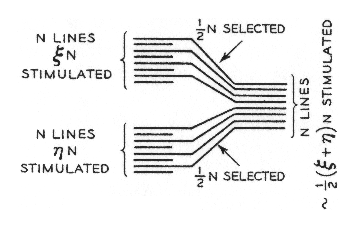
\includegraphics[width=3.2in]{fig_40}
\caption{\label{fig:40}}
\end{figure}

\begin{figure}[b]
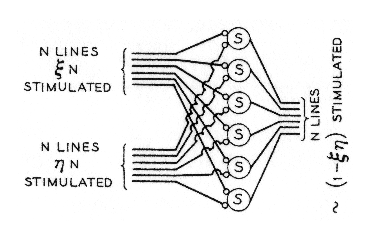
\includegraphics[width=3.2in]{fig_41}
\caption{\label{fig:41}}
\end{figure}

\subsection{\label{sec:twelve3}Discussion of the Algebraical Calculus Resulting from the Above Operations}

Thus our present analog system can be used to build up a system of
algebra where the fundamental operations are

\begin{eqnarray}
\label{eq:31} \begin{array}{ll}\left\{\begin{array}{l}
\left\begin{array}{l}
\alpha\\
\alpha\xi+(1-\alpha)\eta
\end{array}\right\}\\
1-\xi\eta
\end{array}\right
&\begin{array}{l}\left\{\begin{array}{l} $(for any constant$~\alpha\\
$in$~0\leq\alpha\leq1)~,
\end{array}
\\\\
\end{array}
\end{array}
\end{eqnarray}

\noindent All these are to be viewed as functions of $\xi$,
$\eta$. They lead to a system, in which one can operate freely
with all those functions $f(\xi_1,\xi_2,\ldots,\xi_k)$ of any $k$
variables $\xi_1,\xi_2,\ldots,\xi_k$, that the functions of
Eq.~\ref{eq:31} generate. I.e., with all functions that can be
obtained by any succession of the following processes:

\renewcommand{\labelenumi}{\Alph{enumi}}

\begin{enumerate}
    \item In the functions of Eq.~\ref{eq:31} replace $\xi$,
    $\eta$ by any variables $\xi_i$, $\xi_j$.
    \item In a function $f(\xi_1^*,\ldots,\xi_\ell^*)$, that has
    already been obtained, replace the variables
    $\xi_1^*,\ldots,\xi_\ell^*$, by any functions
    $g_1(\xi_1,\ldots,\xi_k),\ldots,g_\ell(\xi_1,\ldots,\xi_k)$,
    respectively, that have already been obtained.
\end{enumerate}

\noindent To these, purely algebraical-combinatorial processes we
add a properly analytical one, which seems justified, since we
have been dealing with approximative procedures, anyway:

\begin{enumerate}
\addtocounter{enumi}{2}
    \item  If a sequence of functions $f_u(\xi_1,\ldots,\xi_k)$,
    $u=1,2,\ldots$, that have already been obtained, converges
    uniformly (in the domain
    $0\leq\xi_1\leq1,\ldots,0\leq\xi_k\leq1$) for
    $u\rightarrow\infty$ to $f(\xi_1,\ldots,\xi_k)$, then form
    this $f(\xi_1,\ldots,\xi_k)$.
\end{enumerate}

Note, that in order to have the freedom of operation as expressed
by (A), (B), the same ``randomness" conditions must be postulated
as in the corresponding parts of sections \ref{sec:nine} and
\ref{sec:ten}. Hence ``randomizing" permutations \textsf{U} must
be interposed between consecutive executive organs (i.e., those
described above and re-enumerated in (A)), just as in the sections
referred to above.

In ordinary algebra the basic functions are different ones,
namely:

\begin{eqnarray}
\label{eq:32} \begin{array}{ll}\left\{\begin{array}{l}
\left\begin{array}{l}
\alpha\\
\xi+\eta
\end{array}\right\}\\
\xi\eta
\end{array}\right
&\begin{array}{l}\left\{\begin{array}{l} $(for any constant$~\alpha\\
$in$~0\leq\alpha\leq1)~,
\end{array}
\\\\
\end{array}
\end{array}
\end{eqnarray}

It is easily seen, that the system Eq.~\ref{eq:31} can be
generated (by (A), (B)) from the system Eq.~\ref{eq:32}, while the
reverse is not obvious (not even with (C) added). In fact
Eq.~\ref{eq:31} is intrinsically more special than
Eq.~\ref{eq:32}, i.e., the functions that Eq.~\ref{eq:31}
generates are fewer than those that Eq.~\ref{eq:32} generates
(this is true for (A), (B), and also for (A), (B), (C)) - the
former do not even include $\xi+\eta$. Indeed all functions of
Eq.~\ref{eq:31}, i.e., of (A) based on Eq.~\ref{eq:31}, have this
property: If all variables lie in the interval $0\leq\xi\leq1$,
then the function, too, lies in that interval. This property is
conserved under the applications of (B), (C). On the other hand
$\xi+\eta$ does not possess this property - hence it cannot be
generated by (A), (B), (C) from Eq.~\ref{eq:31}. (Note, that the
above property of the functions of Eq.~\ref{eq:31}, and of all
those that they generate, is a quite natural one: They are all
dealing with excitation levels, and excitation levels must, by
their nature, be numbers $\xi$ with $0\leq\xi\leq1$.)

In spite of this limitation, which seems to mark it as essentially
narrower than conventional algebra, the system of functions
generated (by (A), (B), (C)) from Eq.~\ref{eq:31} is broad enough
for all reasonable purposes. Indeed, it can be shown that the
functions so generated comprise precisely the following class of
functions:

All functions $f(\xi_1,\xi_2,\ldots,\xi_k)$ which, as long as
their variables $\xi_1,\ldots,\xi_k$ lie in the interval
$0\leq\xi\leq1$, are continuous and have their value lying in that
interval too.

We will not give the proof here, it runs along quite conventional
lines.

\subsection{\label{sec:twelve4}Limitations of this System}

This result makes it clear, that the above analog system, i.e.,
the system of Eq.~\ref{eq:31}, guarantees for numbers $\xi$ with
$0\leq\xi\leq1$ (i.e., for the numbers that it deals with, namely
excitation levels) the full freedom of algebra and of analysis.

In view of these facts, this analog system would seem to have
clear superiority over the digital one. Unfortunately, the
difficulty of maintaining accuracy levels counterbalances the
advantages to a large extent. The accuracy can never be expected
to exceed $1/N$. In other words, there is an intrinsic noise level
of the order $1/N$, i.e., for the $N$ considered in
\ref{sec:ten5_2} and \ref{sec:ten5_3} (up to $\sim20,000$) at best
$10^{-4}$. Moreover, in its effects on the operations of
Eq.~\ref{eq:31}, this noise level rises from $1/N$ to
$1/\sqrt{N}$. (E.g., for the operation $1-\xi\eta$, cf. the result
Eq.~\ref{eq:21} and the argument that leads to it.) With the above
assumptions, this is at best $\sim10^{-2}$, i.e., $1\%$! Hence
after a moderate number of operations, the excitation levels are
more likely to resemble a random sampling of numbers than
mathematics.

It should be emphasized, however, that this is not a conclusive
argument that the human nervous system does not utilize the analog
system. As was pointed out earlier, it is in fact known for at
least some nervous processes that they are of an analog nature,
and that the explanation of this may, at least in part, lie in the
fact that the ``logical depth" of the nervous network is quite
shallow in some relevant places. To be more specific: The number
of synapses of neurons from the peripheral sensory organs, down
the afferent nerve fibres, through the brain, back through the
efferent nerves to the motor system may not be more than $\sim10$.
Of course the parallel complexity of the network is indisputable.
``Depth" introduced by feedback in the human brain may be overcome
by some kind of self-stabilization. At the same time, a good
argument can be put up that the animal nervous system uses analog
methods (as they are interpreted above) only in the crudest way,
accuracy being a very minor consideration.

\subsection{\label{sec:twelve5}A Plausible Analog Mechanism: Density Modulation by Fatigue}

\begin{figure}
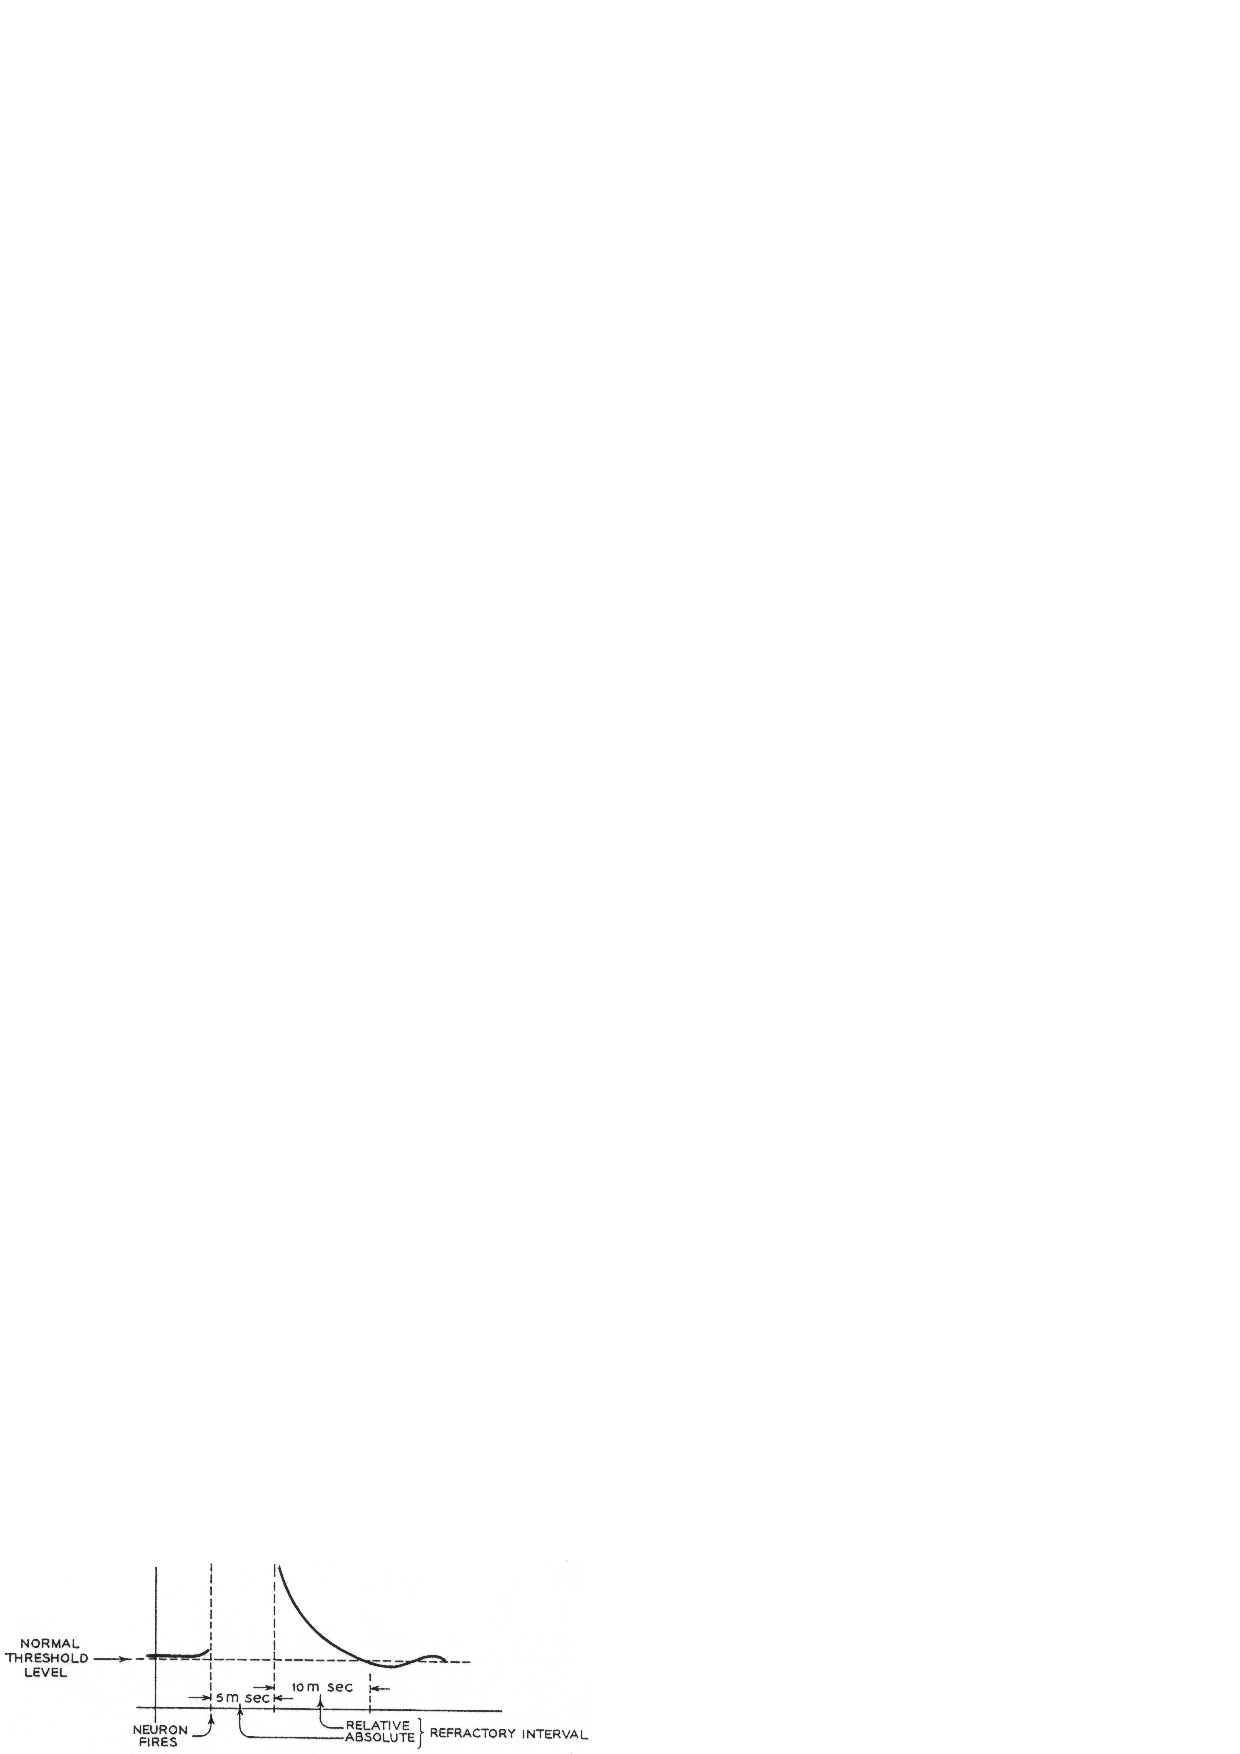
\includegraphics[width=3.4in]{fig_42}
\caption{\label{fig:42}}
\end{figure}

Two more remarks should be made at this point. The first one deals
with some more specific aspects of the analog element in the
organization and functioning of the human nervous system. The
second relates to the possibilities of stabilizing the precision
level of the analog procedure that was outlined above.

This is the first remark. As we have mentioned earlier, many
neurons of the nervous system transmit intensities (i.e.,
quantitative data) by analog methods, but, in a way entirely
different from the method described in \ref{sec:twelve2},
\ref{sec:twelve3} and \ref{sec:twelve4}. Instead of the level of
excitation of a nerve (i.e., of a bundle of nerve fibres) varying,
as described in \ref{sec:twelve2}, the single nerve fibres fire
repetitiously, but with varying frequency in time. For example,
the nerves transmitting a pressure stimulus may vary in frequency
between, say, 6 firings per second and, say, 60 firings per
second. This frequency is a monotone function of the pressure.
Another example is the optic nerve, where a certain set of fibres
responds in a similar manner to the intensity of the incoming
light. This kind of behavior is explained by the mechanism of
neuron operation, and in particular with the phenomena of
threshold and of fatigue. With any peripheral neuron at any time
can be associated a threshold intensity: A stimulus will make the
neuron fire if and only if its magnitude exceeds the threshold
intensity. The behavior of the threshold intensity as a function
of the time after a typical neuron fires is qualitatively pictured
in Figure~\ref{fig:42}. After firing, there is an ``absolute
refractory period" of about 5 milliseconds, during which no
stimulus can make the neuron fire again. During this period, the
threshold value is infinite. Next comes a ``relative refractory
period" of about 10 milliseconds, during which time the threshold
level drops back to its equilibrium value (it may even oscillate
about this value a few times at the end). This decrease is for the
most part monotonic. Now the nerve will fire again as soon as it
is stimulated with an intensity greater than its excitation
threshold. Thus if the neuron is subjected to continual excitation
of constant intensity (above the equilibrium intensity), it will
fire periodically with a period between 5 and 15 milliseconds,
depending on the intensity of the stimulus.

Another interesting example of a nerve network which transmits
intensity by this means is the human acoustic system. The ear
analyzes a sound wave into its component frequencies. These are
transmitted to the brain through different nerve fibres with the
intensity variations of the corresponding component represented by
the frequency modulation of nerve firing.

The chief purpose of all this discussion of nervous systems is to
point up the fact that it is dangerous to identify the real
physical (or biological) world with the models which are
constructed to explain it. The problem of understanding the animal
nervous action is far deeper than the problem of understanding the
mechanism of a computing machine. Even plausible explanations of
nervous reaction should be taken with a very large grain of salt.

\subsection{\label{sec:twelve6}Stabilization of the Analog System}

\begin{figure}[t]
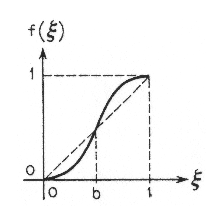
\includegraphics[width=2.4in]{fig_43}
\caption{\label{fig:43}}
\end{figure}

We now come to the second remark. It was pointed out earlier, that
the analog mechanism that we discussed may have a way of
stabilizing excitation levels to a certain precision for its
computing operations. This can be done in the following way.

For the digital computer, the problem was to stabilize the
excitation level at (or near) the two values 0 and 1. This was
accomplished by repeatedly passing the bundle through a simple
mechanism which changed an excitation level $\xi$ into the level
$f(\xi)$, where the function $f(\xi)$ had the general form shown
in Figure~\ref{fig:43}. The reason that such a mechanism is a
restoring organ for the excitation levels $\xi\sim0$ and
$\xi\sim1$ (i.e., that it stabilizes at - or near - 0 and 1) is
that $f(\xi)$ has this property: For some suitable $b(0\leq
b\leq1)$, $0<\xi<b$ implies $0<f(\xi)<\xi$; $b<\xi<1$ implies
$\xi<f(\xi)<1$. Thus $\xi=0,1$ are the only stable fixpoints of
$f(\xi)$. (Cf. the discussion in \ref{sec:nine2_3} and
\ref{sec:nine4_2}.)

\begin{figure}[t]
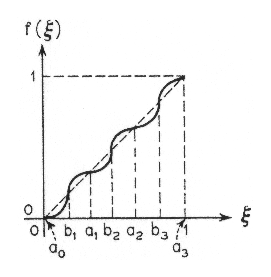
\includegraphics[width=2.4in]{fig_44}
\caption{\label{fig:44}}
\end{figure}

Now consider another $f(\xi)$, which has the form shown in
Figure~\ref{fig:44}. I.e., we have:

\begin{eqnarray*}
\begin{array}{l}
0=a_0<b_1<a_1,<\ldots<a_{\nu-1}<b_\nu<a_\nu=1~,\\
$for$~i=1,\ldots,\nu~:\\\\
~~~a_{i-1}<\xi<b_i \Rightarrow a_{i-1}<f(\xi)<\xi\\
~~~b_i<\xi<a_i \Rightarrow \xi<f(\xi)<a_i~.
\end{array}
\end{eqnarray*}

\noindent Here $a_0(=0),a_1,\ldots,a_{\nu-1},a_\nu(=1)$ are
$f(\xi)$'s only stable fixpoints, and such a mechanism is a
restoring organ for the excitation levels $\xi\sim
a_0(=0),a_1,\ldots,a_{\nu-1},a_\nu(=1)$. Choose, e.g., $a_i=i/\nu$
($i=0,1,\ldots,\nu$), with $\nu^{-1}<\delta$, or more generally,
just $a_i-a_{i-1}<\delta$ ($i=1,\ldots,\nu$) with some suitable
$\nu$. Then this restoring organ clearly conserves precisions of
the order $\delta$ (with the same prevalent probability with which
it restores).

\section{\label{sec:thirteen}Concluding Remark}

\subsection{\label{sec:thirteen1}A Possible Neurological Interpretation}

There remains the question, whether such a mechanism is possible,
with the means that we are now envisaging. We have seen further
above, that this is the case, if a function $f(\xi)$ with the
properties just described can be generated from Eq.~\ref{eq:31}.
Such a function can indeed be so generated. Indeed, this follows
immediately from the general characterization of the class of
functions that can be generated from Eq.~\ref{eq:31}, discussed in
\ref{sec:twelve3}. However, we will not go here into this matter
any further.

It is not inconceivable that some ``neural pools" in the human
nervous system may be such restoring organs, to maintain accuracy
in those parts of the network where the analog principle is used,
and where there is enough ``logical depth" (cf. \ref{sec:twelve4}
to make this type of stabilization necessary.

\section{Acknowledgements}

Retyped in \LaTeX by Akram S. Sadek, 22 March 2005.

\bibliography{vN_prob_logics}


\end{document}
